%!TEX root = ../template.tex
%%%%%%%%%%%%%%%%%%%%%%%%%%%%%%%%%%%%%%%%%%%%%%%%%%%%%%%%%%%%%%%%%%%%
%% chapter2.tex
%% NOVA thesis document file
%%
%% Chapter with the template manual
%%%%%%%%%%%%%%%%%%%%%%%%%%%%%%%%%%%%%%%%%%%%%%%%%%%%%%%%%%%%%%%%%%%%

\typeout{NT FILE chapter2.tex}%

\chapter{Related Work}
\label{cha:related_work}

\section{Introduction}
\label{sec:introduction}

In order to design a sensing system, it is important to determine the type of sensor to be used. This choice has to address the challenges presented by the environment in which the experience is conducted, as well as the goals of the experiment itself. The evaluation of several types of sensors in Subsection \ref{subsec:sensing_technologies} provides context for the decision to use the \gls{FMCW} radar for human motion detection in this thesis. Its operation is briefly explained in Subsection \ref{subsec:fmcw_operation_overview}.

\gls{ML} is the process of extracting patterns from data to make decisions, and it is a very appealing solution to complex problems that entices researchers from a variety of communities to use it in their projects \cite{MLprospects_ch2intro}. However, as technology has advanced, datasets have grown larger and more complex, requiring faster analysis. Raw data must be transformed into meaningful features that represent specific properties of the observations before ML algorithms can be applied. This process, known as \textit{feature engineering}, is crucial to the success of machine learning \cite{ch2intro_featureEngineering}. \\
Since \gls{ML} has a wide range of applications, each with different characteristics, there is no standard approach to feature engineering, thus, it is important to experiment with different techniques and observe their effects on model performance. Sections \ref{sec:featureEngineering} and \ref{sec:machine_learning_techniques} summarize features engineering and ML topics, respectively. 

\subsection{Sensing Technologies}
\label{subsec:sensing_technologies}

When it comes to motion and gesture sensing, there are several types of sensors to be considered. They can be divided into wearable and non-wearable sensors. The first can gather data with high resolution from body movements, namely their acceleration, angular velocity, and displacement \cite{SOA_FMCW_biLSTM},  but they have one critical limitation: their practicality. This is due to the fact that to recognize a gesture, the participant needs to be wearing the said device, \cite{FMCWtempofeature}. Accelerometers and gyroscopes are examples of wearable sensors.
On the other hand, non-wearable sensors do not have this limitation and can have the upper hand regarding battery life duration \cite{SOA_FMCW_biLSTM}. Furthermore, the technology needs to be user-friendly and functional when the user is responsible for operating the equipment. Non-wearable sensors combine those characteristics and can include cameras, radars, infrared, ultrasonic, and laser sensors. A brief overview of these sensing alternatives is discussed in the following paragraphs.
\textbf{Cameras} have advanced over time in terms of resolution and this qualifies them as an excellent option for sensing systems, since pictures or frames with better quality, almost directly imply a better performance in gesture recognition solutions \cite{IETBiometricsCameras}. However, there is a tradeoff between this and their sensitivity to light conditions and inaptitude to capture images in cases of occlusion. Therefore, most studies using them take place indoors. Not only that but in cases where privacy is valued, cameras might not be the best option since they compromise the identity of the subject.

In the case of \textbf{Infrared} sensors, the broad \gls{FoV} is one of their characteristics. Their drawbacks include that they operate only at small distances and that meteorological conditions can negatively affect their performance.

\textbf{Ultrasonic sensors} can be used to measure an object's distance based on the time interval it takes for an emitted wave to be sent and reflected. They operate on a higher range of frequencies, higher than the range of human hearing, and the waves emitted are faster than the speed of light. Using these types of sensors rules out limitations like colour and transparency of objects, and light and environment conditions such as  dust, dirt, or high-moisture \cite{ultrasonic}. However, the temperature can negatively affect their performance \cite{ultrasonicRadar}, as well as certain softer, smaller or curvier objects.

Using \textbf{LiDAR} (Light Detection and Ranging) technology has many advantages, including the precision and accuracy obtained in the distance measurements acquired using a pulsed laser. Using this form of range estimation gives excellent results at larger distances, the only setback is the computational power required to make this solution feasible.

In addition, \textbf{Radar} can also be used for sensing, and it is the technology employed for the purpose of this thesis. Distances to objects nearby can be obtained given the \gls{ToF}, which estimates the time it takes for a radar wave to be sent and reflected back to the radar. Unlike the previously mentioned, the radar performs great under challenging meteorological and lighting conditions, and it can even work in cases of occlusion, penetrating most  materials. It respects the users' privacy and can easily be integrated into objects while remaining discrete and not taking away from their aesthetic appeal. However, object classification in radar-based systems still faces many challenges despite its great potential.

\section{Fundamentals of FMCW Operation}
\label{sec:fundamentals_fmcw_operation}
\subsection{History of Radar}
\label{history}
A radar device can detect obstacles by emitting a \gls{RF} signal and estimating the time it takes for it to be reflected by an object's surface. By studying the characteristics of the received signal, it's possible to gather information about these objects, such as their speed and the distance at which they stand, hence the name \gls{RADAR}.\\
Radar's development path dates back to the 19th century, when Heinrich Hertz realized radio waves suffered some kind of interference due to metallic obstacles in their way. Outing that information amongst the scientific community led to Nikola Tesla stating his theory for that matter. In his words, "When we raise the voice and hear an echo in reply, we know that the sound of the voice must have reached a distant wall or boundary, and must have been reflected from the same. Exactly as the sound, so an electrical wave is reflected, and the same evidence can be used to determine the relative position or course of a moving object such as a vessel at sea" \cite{radarHistory}.\\
But it was not until 1904 that a prototype called Telemobiloscope, developed by Christian Hülsmeye was first demonstrated. It was a simple chip capable of detecting objects even in the presence of fog, although it couldn't determine their range.
During WWII, radar technology was crucial to the Allies' victory and has since undergone many improvements. The credit goes to the british physicist Robert Watson-Watt and his radio research team, who, in the midst of a project for detecting enemy aircraft, came up with the idea for the first pulsed radar to exist globally \cite{fmcwBookJankiraman}.\\
The term RADAR ended up being coined in 1939, and later studies proved that the use of higher frequencies made the radar systems more robust towards weather conditions and that short pulses of radio waves would revolutionize future radar solutions \cite{radarHistory}.\\
Ever since, further study of radar as well as several breakthroughs in areas such as electronics and computing made it possible for physical devices to be smaller, portable, more efficient and sophisticated. Today, this technology is embedded in a vast range of use cases, from health care \cite{radarHealthcare, radarApplications} to building, security and surveillance \cite{radarApplications}, environmental applications \cite{radarEnvironmentalAppli}, aviation, shipping, mapping, and vehicle safety \cite{radarApplicationsIeee}. 

\subsection{FMCW Radar operation overview}
\label{subsec:fmcw_operation_overview}

The \gls{FMCW} radar operates with \gls{CW}, which means it produces a continuous signal, contrary to pulsed radars. Frequency-modulated signals vary their frequency over time, sweeping across a specific bandwidth. Frequency changes are based on the \gls{LFM} waveform, which may be linear sawtooth FM, linear triangular FM or segmented FM, although the first one is the most common, and is represented in Figure \ref{fig:sawtoothLFM}. This signal is produced by the waveform generator, as shown in Figure \ref{fig:fmcw_block_diagram} where a FMCW radar scheme is presented, and it shapes the transmitted signal's frequency in the \gls{VCO}.
 
\begin{figure}
    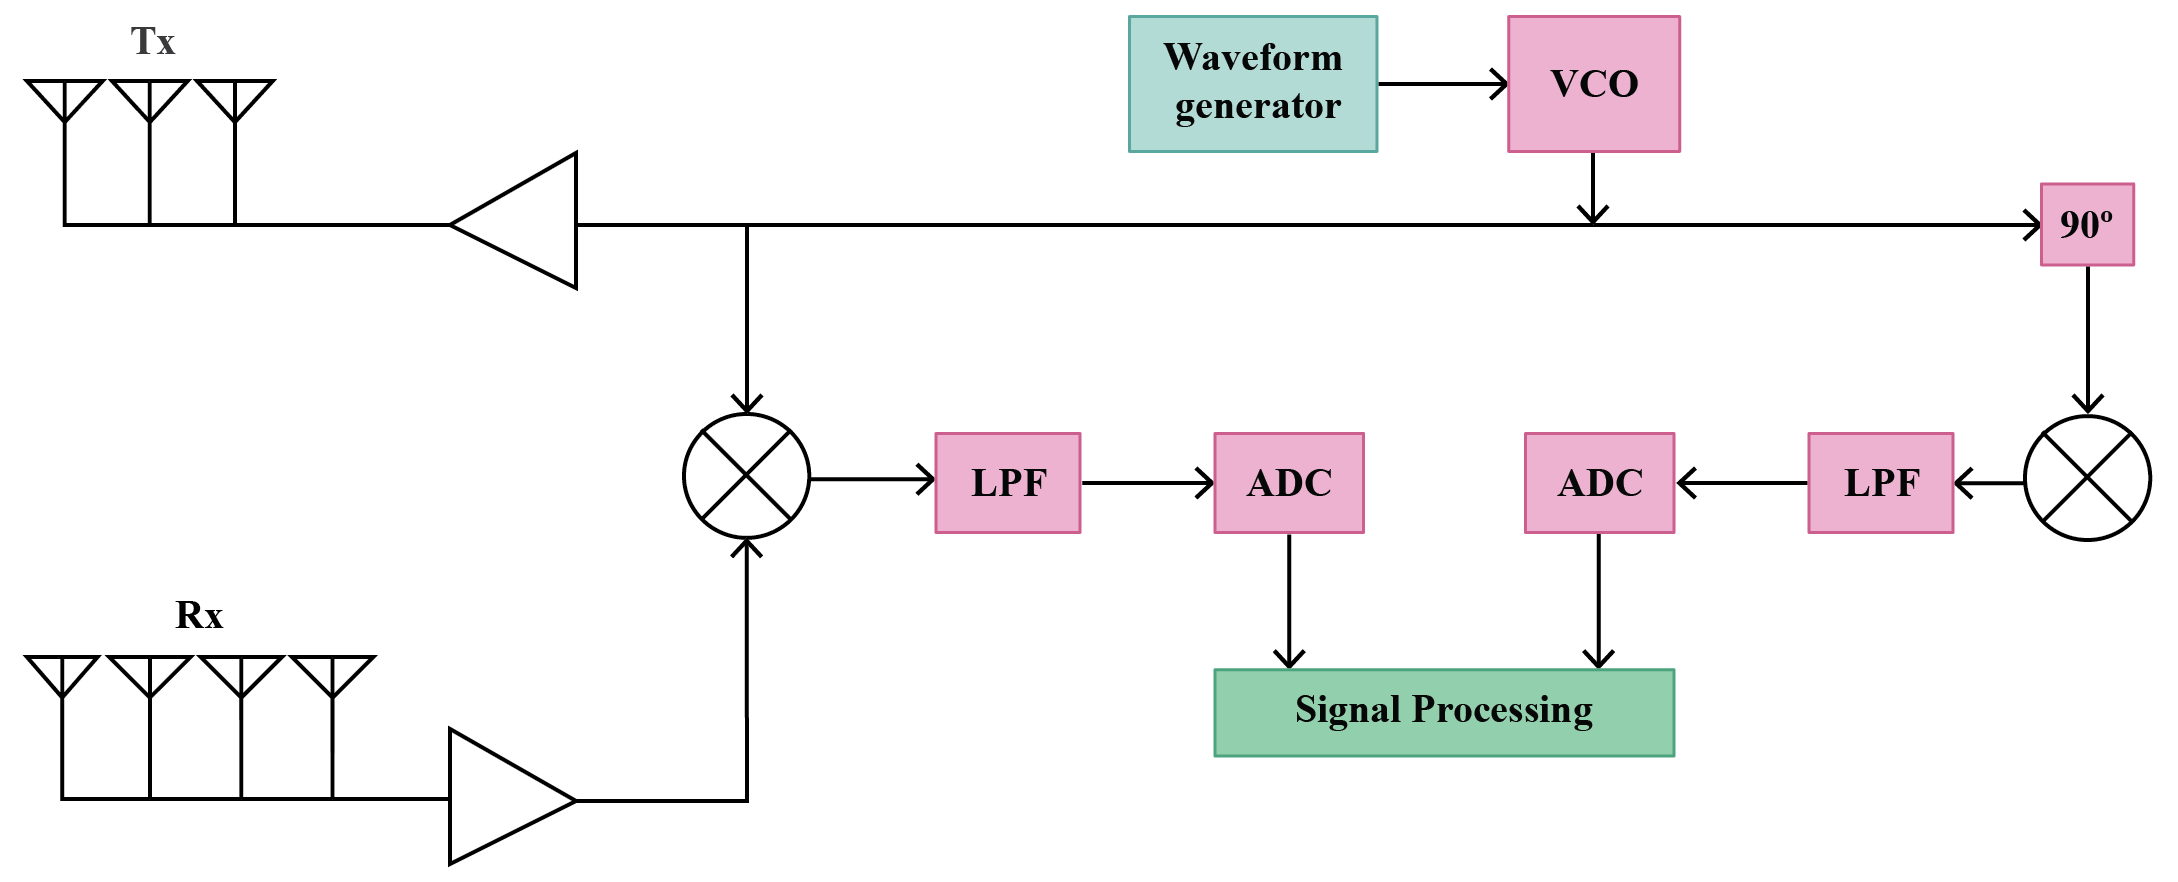
\includegraphics[scale = 0.20]{Chapters/Figures/Block diagram-07.png}
    \caption{FMCW Radar Block Diagram Representation.}
    \label{fig:fmcw_block_diagram}
\end{figure}

\begin{figure}[ht]
        \centerline{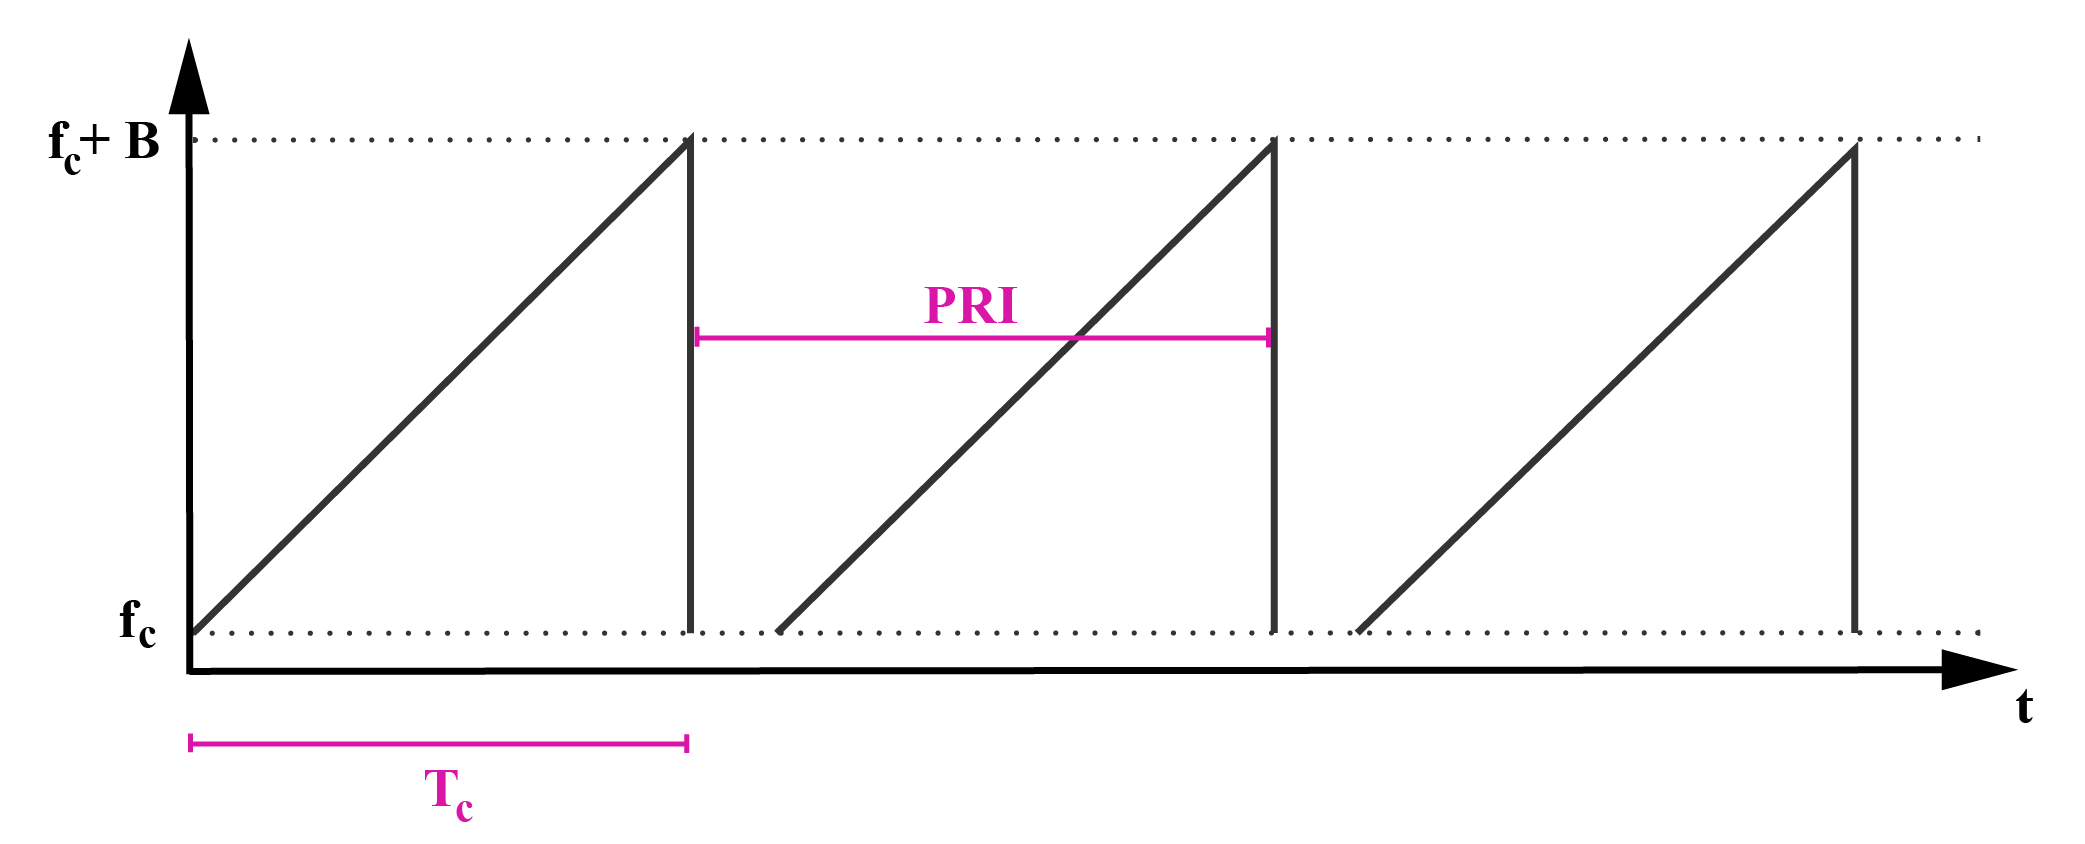
\includegraphics[scale = 0.18]{Chapters/Figures/Sawtooth modulation novo-01.png}}
        \caption{Linear Sawtooth modulation.}
         \label{fig:sawtoothLFM}
\end{figure}  

The bandwidth $B$ is swept periodically during a time period $T_c$, known as \textit{sweep time}, resulting in multiple transmitted \textit{chirps} over time. It is necessary to assure a delay between chirps, in order to eliminate any potential ambiguities when estimating range and velocity later on. In Figure \ref{fig:sawtoothLFM}, the \gls{PRI} encapsulates the period $T_c$ and that delay.
Without modulation, it would not be possible to measure \gls{ToF} in \gls{CW} radars because there would be no way to distinguish between multiple continuous echoes received as a continuous signal is being transmitted. With modulation, the variation in frequency allows the detection of a delay in the reception of these echoes, since the frequency transmitted is different and known at each instant. 

In order to compensate for possible losses along the way, the VCO's signal is amplified before being transmitted. Doing so allows it to reach the desired targets, thus affecting range, and to be reflected with enough power to be detected. Furthermore, the received signal is amplified to make it strong enough for processing, improving the ability to pinpoint subtle variations in frequency, and allowing distance and velocity to be calculated more accurately later on. The linear sawtooth FMCW waveform transmitted by the radar and an example of two echos received as a result of two different targets' reflections can be observed in Figure \ref{fig:radarPrinciple}. 

\begin{figure}[ht]
        \centerline{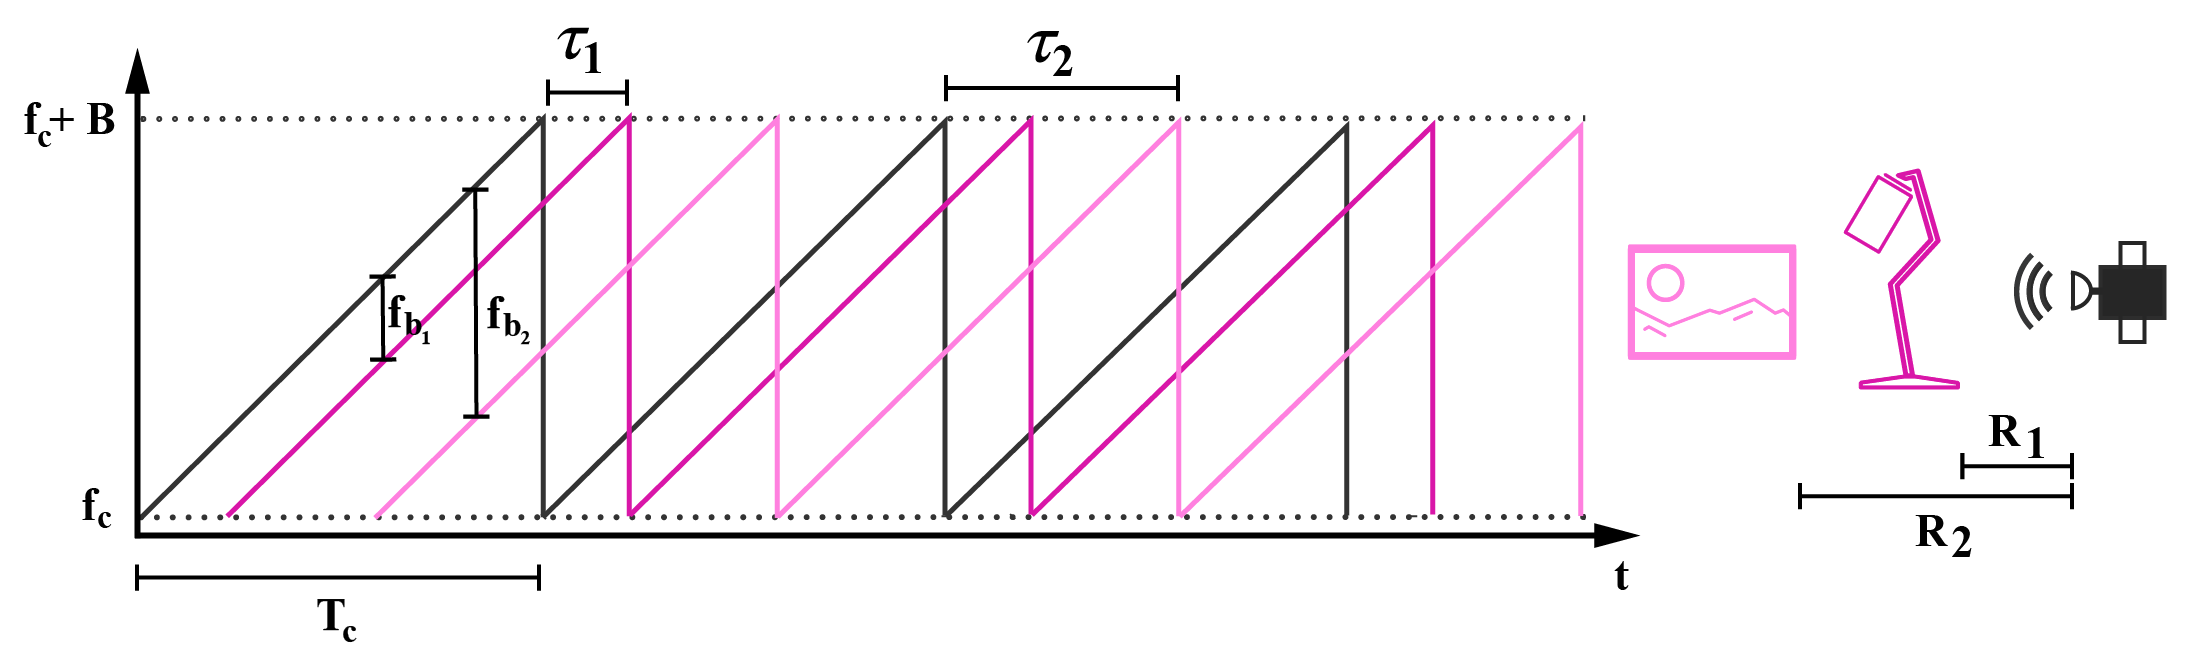
\includegraphics[scale = 0.20]{Chapters/Figures/Radar principle-02-02.png}}
         \caption{a) Linear sawtooth FMCW transmitted waveform in black. Received signals with delay $\tau_1$ and $\tau_2$ in colour, each corresponding to different targets represented in b). b) Two static targets at different ranges from the radar.}
         \label{fig:radarPrinciple}
\end{figure}

By mixing the transmitted and received signals it is possible to obtain the \gls{IF} signal or beat signal, which reflects the difference in frequency of the two caused by \gls{ToF}. This operation is performed recurring to a mixer. 
As we can see from the diagram in Figure \ref{fig:fmcw_block_diagram}, the \gls{IF} signal then passes through a \gls{LPF}, followed by an \gls{ADC}, which will transform the analog signal to a discrete digital signal, at a fixed rate of samples. The digital signal is passed to the \gls{DSP} block, which will then apply a \gls{FFT}. The output of this operation results in a beat frequency spectrum, that can then be used by the radar system to detect and track targets, and measure range and velocity.


\subsection{Measurements}
\label{measurements}
\subsubsection{Distance measurements}
\label{distance_measurements}
For the purpose of this thesis, a sawtooth \gls{LFM} will be considered.
It is possible to define the frequency of each chirp as
\begin{equation}
    \label{eq:tx_freq_reta}
    f(t) = f_{c} + \frac{B}{T_{c}} t,
\end{equation} 
%
with $f_c$ corresponding to the carrier frequency, B the swept bandwidth of each chirp and $T_c$ the period of each chirp. Note that the $B/T_c$ quotient is the frequency sweep rate or chirp rate, represented by the slope of the sawtooth signal.
 
In telecommunications, the standard way to represent a signal is with a cosine function, and a standard signal with an amplitude value of 1 and a null phase can be described as
\begin{equation} \label{eq:standardSignal_cosine}
    A(t) = Acos(2 \pi ft).
\end{equation} 

 Given the block diagram in Figure \ref{fig:fmcw_block_diagram}, the transmitted signal can be written as
 \begin{equation}
    \label{eq:Stx_signal}
     S_{Tx} (t) =  Acos ( 2 \pi (f_c t + \frac{B}{2T_c} t^2)).
 \end{equation}

 Accounting for the delay caused by \gls{ToF}, represented by $\tau$, it is possible to write the echo of the transmitted signal, the received signal, as
 \begin{equation}
    \label{eq:Srx_signal}
     S_{Rx} (t) = Acos ( 2 \pi (f_c (t-\tau) + \frac{B}{2T_c} (t-\tau)^2).
 \end{equation}
 
The \gls{IF} signal is a sinusoidal wave of frequency $f_b$, beat signal frequency, a result of the subtraction of frequency $f_{Tx}$ and $f_{Rx}$. Therefore, the beat signal frequency is given by
\begin{equation}
    \label{eq:beat_frequency_time}
     f_b(t) = f_{Tx}(t) - f_{Rx} (t).
 \end{equation}

To obtain the mentioned \gls{IF} signal, it is necessary to submit the transmitted and received signal to a mixer, which can operate based on a real baseband or a complex-baseband implementation. The first one uses a real mixer and a real baseband architecture, using only the \gls{I} component of the transmitted signal. Therefore, it only uses one ADC chain, and the final output it produces has a more significant performance loss than complex-baseband implementation.\\
The complex-baseband implementation uses a quadrature mixer, using both \gls{I} component and \gls{Q} of the signal produced by the \gls{VCO}, consequently needing two ADC chains. Although it is more expensive than the first solution, the output signal has a better noise-figure ratio \cite{FMCWTexas}. In Figure \ref{fig:mixerComplexBaseband} we can see the representation of complex-baseband implementation, which will be used in the scope of this thesis.

\begin{figure}[ht]
    \centerline{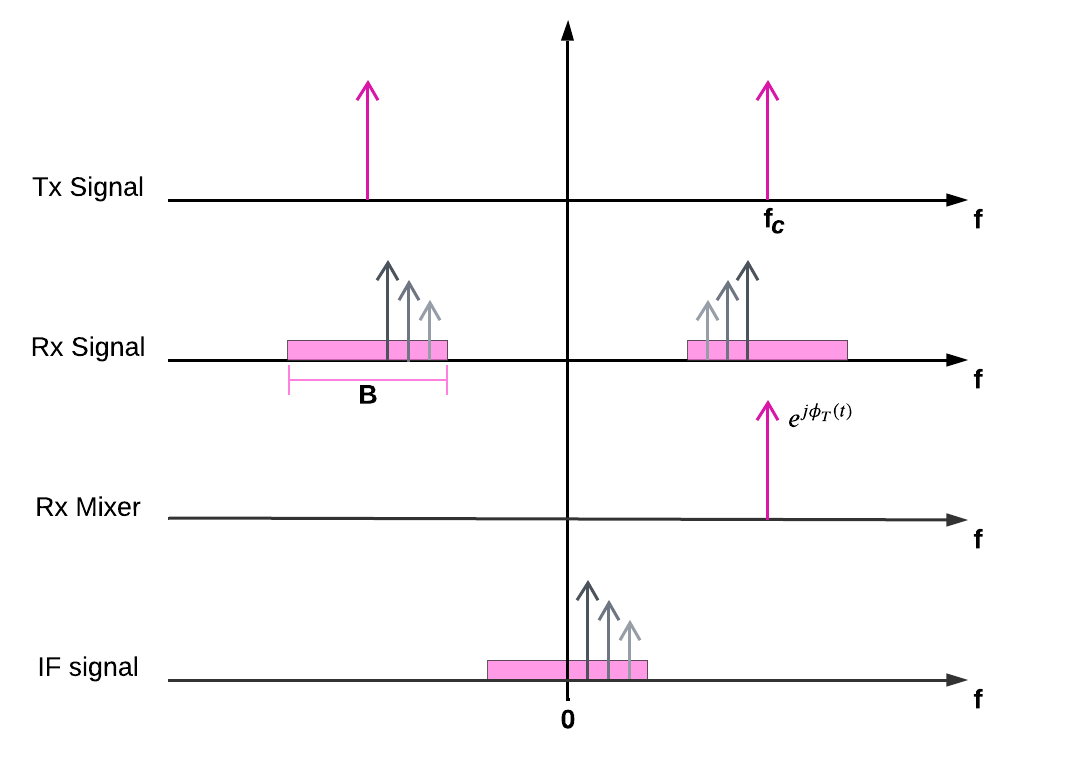
\includegraphics[scale = 0.30]{Chapters/Figures/Radar overview charts - MIXER.png}}
    \caption{Complex-baseband mixer implementation.}
    \label{fig:mixerComplexBaseband}
\end{figure}

The \gls{I} component, $S_{Tx}$, is mixed with the received signal, $S_{Rx}$, as can be described by the following equation, based on \cite{FMCWmixer_equations}

\begin{equation}
    \begin{gathered}
    \label{eq:MixerInPhase}
    S_{Tx} \cdot  S_{Rx} = 
    \frac{A}{2} cos \left ( 2\pi \left (f_c (2t -\tau) + \frac{B}{T_c} \left(t^2 -t\tau + \frac{\tau^2}{2}\right)\right)\right) + \\
    \frac{A}{2} cos \left( 2\pi \left(f_c\tau + \frac{B}{T_c} \left(t\tau - \frac{\tau^2}{2} \right) \right )\right) .
    \end{gathered}
 \end{equation}

 For the second chain of \gls{LPF} and \gls{ADC}, the \gls{Q} component is mixed with the received signal, originating the following expression
 
\begin{equation}
    \begin{gathered}
    \label{eq:MixerQuadrature}
    S_{Tx}^{90º} \cdot  S_{Rx} = \frac{A}{2} sin \left ( 2\pi \left (f_c (2t -\tau) + \frac{B}{T_c} \left(t^2 -t\tau + \frac{\tau^2}{2}\right)\right)\right) + \\
    \frac{A}{2} sin \left( 2\pi \left(f_c\tau + \frac{B}{T_c} \left(t\tau - \frac{\tau^2}{2} \right) \right )\right).
   \end{gathered}
 \end{equation}

 Based on \cite{FMCWmixer_equations}, the first term of both signals will be cancelled either because it is beyond the mixer's cutoff frequency or because \gls{LPF} is applied. So, it is possible to write the \gls{IF} signal as 
 \begin{equation}
    \begin{gathered}
        \label{eq:S_IFrange}
        S_{IF}(t)  =  \exp \left(j2\pi \left( \frac{B\tau t}{T_c} + f_c \tau - \frac{B \tau^2}{2T_c} \right)\right).
   \end{gathered}
 \end{equation}

Finally, it is possible to obtain the beat signal by differentiating the instantaneous phase term of the \gls{IF} signal, obtaining
\begin{equation}
    \begin{gathered}
        \label{eq:beatsignal}
        f_b  =  \frac{d}{dt} \left[ \left( \frac{B\tau t}{T_c} + f_c \tau - \frac{B \tau^2}{2T_c} \right)
        \right] = 
        \frac{B\tau}{T_c}.
   \end{gathered}
 \end{equation}

 The \gls{R} of the target when $\tau$ is known represents the \gls{RTD}. Given the speed of light $c = 299 792 458$ $m/s$ at which the transmitted wave travels, $R$ is defined as
 \begin{equation}
    \begin{gathered}
        \label{eq:Rangesimple}
        R  =  \frac{c \tau}{2}.
   \end{gathered}
 \end{equation}
Given the relation established in (\ref{eq:beatsignal}), we can also rewrite (\ref{eq:Rangesimple}) to obtain the range based on the beat frequency of the \gls{IF} signal, given by
\begin{equation}
    \begin{gathered}
        \label{eq:Range_fb}
        R  =  \frac{c f_b T_c}{2B}.
   \end{gathered}
 \end{equation}

If several targets are considered, a Range \gls{FFT} can be applied for each one to obtain the beat signal frequency. It is also important to note that with multiple targets, range resolution is an important performance parameter that measures the smallest range difference that the radar system can detect, and can be described as
\begin{equation}
    \begin{gathered}
        \label{eq:rangeResolution}
        \Delta R = \frac{c \Delta f_b T_c}{2B} = \frac{c}{2B}.
   \end{gathered}
 \end{equation}

\subsubsection{Velocity measurements}
\label{velocity_measurements}

In addition to range, it is also possible to obtain a moving target's velocity using the FMCW radar. In this case, there will be a frequency shift called the Doppler shift, $f_d$, which according to \cite{velocityRadar} can be determined by
\begin{equation}
    \begin{gathered}
        \label{eq:dopplerShift}
        f_d = \frac{2 v f_c}{c}.
   \end{gathered}
 \end{equation}

The received wave will be shifted upwards if the target is moving towards the radar, or downwards in the opposite case, as we can see in Figure \ref{fig:dopplerShift}.
\begin{figure}[ht]
    \centerline{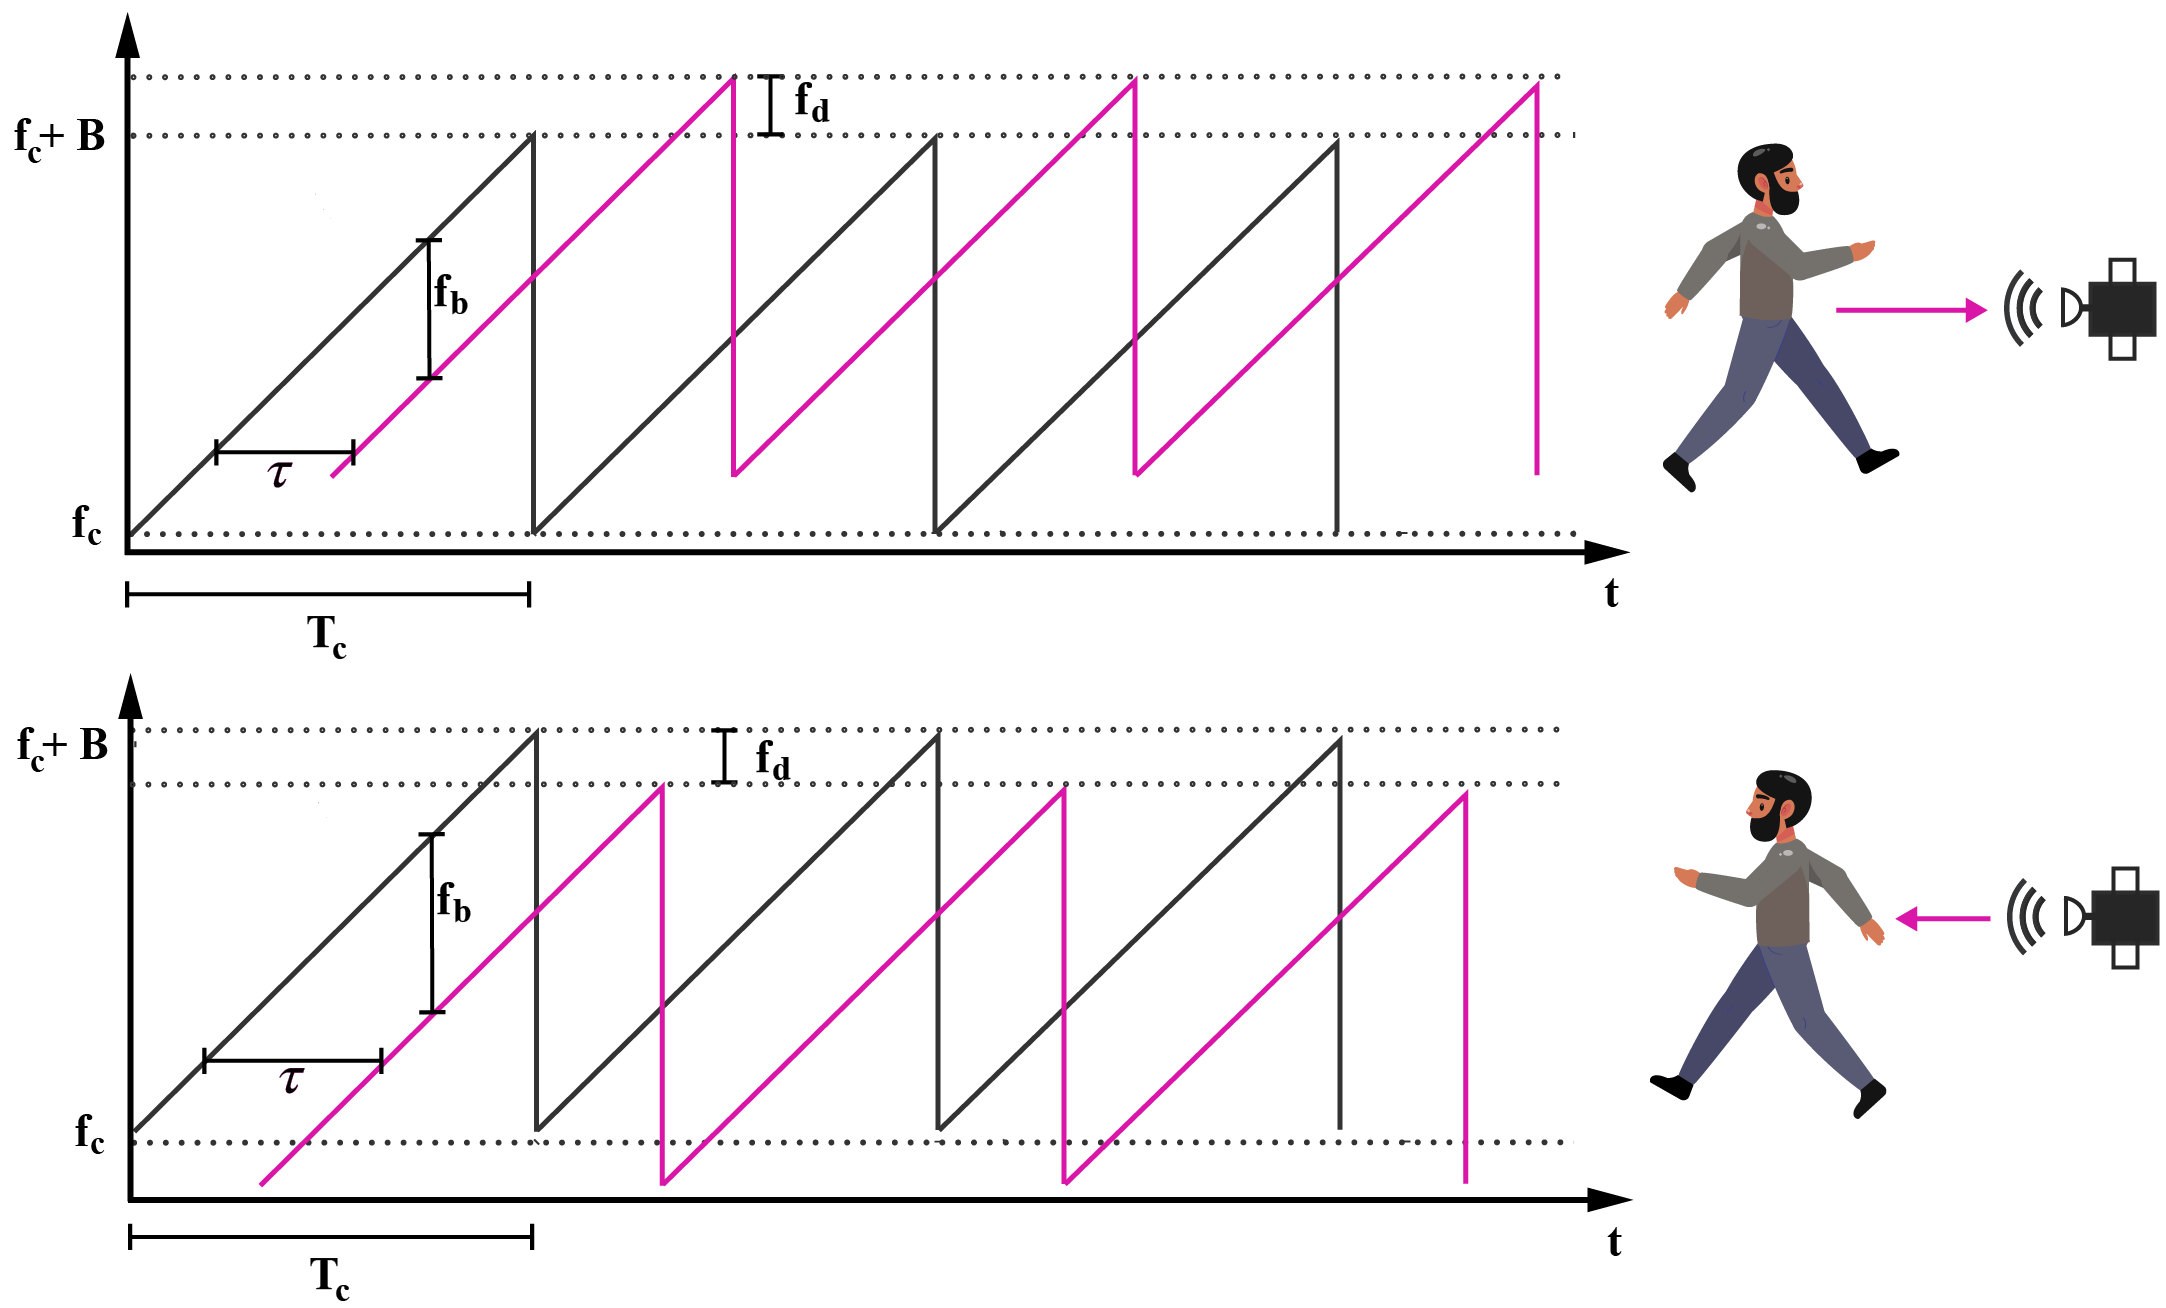
\includegraphics[scale = 0.20]{Chapters/Figures/Radar doppler shift-03.png}}
    \caption{a) Received signal shifted upwards due to Doppler effect of a target moving closer to the radar b) Received signal shifted downwards due to Doppler effect of a target moving away from the radar.}
    \label{fig:dopplerShift}
\end{figure}

In the previous section, it was established that the beat frequency was dependent on the received signal's delay, and in this section it is shown how the Doppler effect also has an impact on that frequency. It is possible to write the received signal's frequency as
\begin{equation}
    \begin{gathered}
        \label{eq:newBeatFrew}
        f_{Rx} = f_c + \frac{B}{T_c} (t - \tau) + f_d.
   \end{gathered}
 \end{equation}
 
The received signal resultant of the reflection on a moving target can be written as
\begin{equation}
    \begin{gathered}
        \label{eq:SRxMovingTarget}
        S_{Rx} = \cos \left(  2\pi\left( (f_c + f_d ) (t- \tau) + \frac{B}{Tc} \left(\frac{t^2}{2} - \tau t\right) + f_d (t- \tau)\right)\right).
   \end{gathered}
 \end{equation}
 
 Recalling (\ref{eq:beatsignal}) and (\ref{eq:dopplerShift}), it is possible to obtain the \gls{IF} signal similarly as before, resulting in the following expression
\begin{equation}
    \begin{gathered}
        \label{eq:IFsignalMovement}
        S_{IF}(t)  =  \exp \left(j2\pi \left( \left(\frac{B\tau }{T_c} + \frac{2v}{c}f_c\right)t+ f_c \tau - \frac{B \tau^2}{2T_c} \right)\right).
   \end{gathered}
 \end{equation}

As depicted in Subsection \ref{subsec:fmcw_operation_overview}, the \gls{DSP} block will perform \gls{FFT} operations to the collected data samples in order for it to be possible to obtain range and velocity information.
The first \gls{FFT} is performed column-wise, making it possible to obtain range information from what it is called a Range Map or Range Profile, a matrix with dimension N x M, where M is the number of chirps transmitted and N is the number of samples. This first transformation can therefore also be denoted as Range FFT. \\
However, according to \cite{velocityRadar}, in the case of moving targets, the amplitude and frequency of each of the IF signals will be similar, and therefore not relevant in determining the targets' velocity. On the other hand, the phase of \gls{IF} signals will suffer slight changes during time, and by applying a row-wise \gls{FFT} to the Range Map previously mentioned, it is possible to obtain a Doppler Spectrum or Range-Doppler profile that contains relevant information for velocity measurement. This second transformation can also be denoted as Doppler FFT.\\
As stated in the previous paragraph, a phase difference can be observed between IF signals, and it is described as in (\ref{eq:phase_diff_movingtargets}). Based on that expression, it is also possible to obtain radial velocity as it is defined in (\ref{eq:radial_velocity}).

\begin{equation}
    \label{eq:phase_diff_movingtargets}
      \Delta \omega_v = 2 \left(\frac{2\pi v T_c}{\lambda} \right),
\end{equation}

\begin{equation} \label{eq:radial_velocity}
    v = \frac{\lambda \Delta \omega_v }{4\pi T_c}. 
\end{equation}

Given (\ref{eq:radial_velocity}) and accounting that phase resolution is limited to $\Delta \omega_v = 2\pi / N_p$ \cite{velocityRadar}, and the velocity resolution can be described as

\begin{equation} \label{eq:20equation}
    \Delta V = \frac{\lambda}{2NT_c}.
\end{equation}

\section{Feature Engineering}
\label{sec:featureEngineering}
In general, a feature is a distinctive aspect of an observed phenomenon that sets it apart in some way. In the scope of \gls{ML}, a feature is a measurable attribute of a phenomenon under study. The selection of appropriate features for use in a machine learning model is crucial for achieving good performance, as the model's ability to learn and make accurate predictions is reliant on the features provided to it. 

Features used in \gls{ML} can be classified into various categories based on their characteristics, such as whether they are numeric or categorical, and how they are obtained, such as being directly extracted from a data series or derived from other features. Features can also be divided based on their domain, and the subsequent paragraphs will discuss both time-domain and frequency-domain features, which are both numerical.

\subsection{Time-Domain Features}
\label{subsec:timeDomainFeatures}
Time domain features are derived from time series data, which consist of a series of data points collected over a period of time. The signals received by the radar are in the time domain before being submitted to a \gls{FFT}, and therefore it is possible to extract several features such as:

\begin{description}

    \item[Peak to Peak value (PP)]  
    The \gls{PP} value of a signal is the difference between the highest and lowest points of a signal over a period of time. It is often used to characterize the overall size or amplitude of the signal $x(t)$, and its expression is given by: 
    \begin{equation} \label{eq:pp}
     PP = | max(x(t)) - min (x(t))|.
    \end{equation}
    
    \item[Standard Deviation (SD)] 
    \gls{SD} is a statistical measure used to quantify the amount of variation or dispersion in a dataset, and it is the square root value of \gls{Var}. It is useful in determining the extent to which the data values in a dataset deviate from the average value of the dataset, meaning the smaller the \gls{SD} value the closer the data is to the mean of the dataset. It can also be used to compare the dispersion of different datasets, and it is a more intuitive measure than  \gls{Var}. \gls{SD} is described as
    \begin{equation} \label{eq:stdDeviation}
     SD = \sqrt{ \frac{1}{N} \sum_{i=1}^{N} (x_i - \overline{x}^2)   }.
    \end{equation}

    \item[Covariance (COV)]  
      can be useful to assess the relationship between two variables, measuring how they change in respect to one another. A negative covariance means the growth of one variable translates into the decrease of the other. Conversely, a positive covariance reflects two variables that grow alongside one another. When the covariance is zero, there is no established relation between the two. \gls{COV} is determined by
    \begin{equation} \label{eq:covariance}
     COV (X, Y) = \frac{1}{N} \sum_{i=1}^{N} (x_i - \overline{x}) (y_i - \overline{y}).
    \end{equation}
  
    \item[Root mean square (RMS)]  
      is often used to describe the effective or average power of a time-varying signal and is also denoted as the quadratic mean, as it's defined by the square root of the mean of the squares of the dataset's values, as follows
    \begin{equation} \label{eq:rms}
     RMS = \sqrt{ \frac{1}{N} \sum_{i=1}^{N} x_i^2  }.
    \end{equation}    

    \item[N-th Raw Moment ($\mu'_n$)]  
    Raw moments are meausures related to the shape and tendency of a distribution. The first four raw moments are mean, variance or standard deviation, skewness and Kurtosis value, respectively. The expression for the n-th raw moment is given by
     \begin{equation} \label{eq:nRawMoment}
     \mu'_n =  \frac{1}{N} \sum_{i=1}^{N} x(i)^n,
     \end{equation}    
    where $x_i$ represents a sample of the dataset, and N represents the size of the fixed window of samples.
    
    \item[N-th Central Moment ($\mu_n$)]  
    Central moments are normalized versions of raw moments and are generally preferred because they are more robust to changes in scale compared to raw moments. They are defined as
     \begin{equation} \label{eq:nCentralMoment}
     \mu'_n =  \frac{1}{N} \sum_{i=1}^{N} (x(i)- \mu'_1)^n ,
     \end{equation}    
    where $x_i$ represents a sample of the dataset, N represents the size of the fixed window of samples, and $\mu'_1$ represents the first raw moment, or in other terms, the mean value.
    
    \item[Magnitude (M) and Phase ($\Phi$)]  
    of the \gls{I} and \gls{Q} signals are defined as 
    \begin{equation} \label{eq:magnitude}
     M = \sqrt{I^2 + Q^2},
    \end{equation}
    \begin{equation} \label{eq:phase}
     M = \arctan \left(\frac{Q}{I}\right).
    \end{equation}

    \item[Discrete Cross-Correlation]  
    In signal processing, it is a common measure of the similarity between two signals. It can be useful to identify patterns in data, and understand the relationship between different signals. It can be described as
    \begin{equation} \label{eq:crossCorrelation}
     \hat{r}_{xy}(k) = \frac{1}{M} \sum_{m=0}^{M-1} x(m) y^*(m+k),
    \end{equation}
     where M is the length of the cross-correlation and $x(m)$ and $y^*(m)$ are the amplitude and conjugate amplitude of the sampled signals at time $m$.
    
    \item[Crest Factor] is a measure of the peak-to-average power ratio of a signal. It is often used to evaluate the amount of distortion that a system or process introduces when processing a signal, it is defined as
    \begin{equation} \label{eq:crest factor}
     CRF = \frac{PP  }{RMS  }.
    \end{equation}


\end{description}


\subsection{Frequency-Domain Features}
\label{subsec:FrequencyDomainFeatures}
As previously stated, \gls{FFT} will be applied to the \gls{IQ} signals, enabling the extraction of frequency-domain features such as the ones we will discuss in this section. It is worth noting that spectral leakage may introduce noise into the spectrum and decrease frequency resolution for the following measurements of range and velocity, but this can be mitigated by selecting an appropriate window size prior to performing the \gls{FFT} \cite{windowFunctionsSpectralLeakage}. An alternative method is to use tailored window functions on the signal, such as the Hanning and Hamming windows, the first of which is successful in 95\% of cases, according to \cite{windowFFTS}.

\begin{description}

    \item[Power Spectral Entropy (PSE)]    
    This feature plays an important role in designing and optimising wireless communication systems because it relates to the amount of data transmitted over a given bandwidth, describing how the power of a signal is distributed over frequency. The Power Spectral Density function is denoted by $\hat{P}(w_i)$ and is defined in (\ref{eq:powerSpectralDensity}). Its distribution function is given by \ref{eq:powerSpectralDistribution}. With those two functions, it is possible to define \gls{PSE} as in (\ref{eq:powerSpectralEfficiency}).
    \begin{equation} \label{eq:powerSpectralDensity}
     \hat{P}(w_i) = \frac{1}{L} | X (w_i) |^2,
    \end{equation}
    \begin{equation} \label{eq:powerSpectralDistribution}
     \hat{P}(w_i) =  \frac{\hat{P}(w_i)}{\sum_{i=1}^{L} \hat{P}(w_i)},
    \end{equation}
        \begin{equation} \label{eq:powerSpectralEfficiency}
     \hat{P}(w_i) =  - \sum_{i=1}^{L} p_i \log p_i.
    \end{equation}
    
\end{description}

The work in \cite{SOA_1DFFT_freqFeatures} was able to bypass complexities such as extensive signal processing and latency by extracting some range-based statistical features from the 1D range FFT plot, such as the \textbf{height}, \textbf{width} and \textbf{area under peaks}, as well as \textbf{peak standard deviation}.\\
    
The \textbf{magnitude based features} presented below proved to be helpful in the detection of six specific hand movements using a CMOS Radar, as described in \cite{SOA_Magnitude_Phase_Features}. They can be derived after applying a \gls{2D-FFT} to the signals received from the \gls{ADC} component, recurring to a \gls{RDI} based on the magnitude of the complex 2D \gls{FFT}, with $Z_i$, $R_i$ and $D_i$ corresponding to the magnitude, range and doppler values of each index $i$ from \gls{RDI} image \cite{SOA_Magnitude_Phase_Features}. They are described as

\begin{description}
    \item[Weighted Range] 
    \begin{equation} \label{eq:weightedRange_ft}
     U = \frac{\sum_{i} Z_i.R_i}{\sum_{i} Z_i},
    \end{equation}

    \item[Weighted Doppler] 
    \begin{equation} \label{eq:weightedDoppler_ft}
     V = \frac{\sum_{i} Z_i.D_i}{\sum_{i} Z_i},
    \end{equation}

    \item[Instantaneous Energy] 
    \begin{equation} \label{eq:instantaneousEnergy_ft}
    I = \sum_{i} Z_i,
    \end{equation}

    \item[Range Dispersion] 
    \begin{equation} \label{eq:rangeDispersion_ft}
     RD = \sqrt{ \frac{ \sum{i} Z_i.(R_i-U)^2 } {\sum{i} Z_i} },
    \end{equation}

    \item[Doppler Dispersion] 
    \begin{equation} \label{eq:dopplerDispersion_ft}
     DD = \sqrt{ \frac{ \sum{i} Z_i.(R_i-V)^2 } {\sum{i} Z_i} }.
    \end{equation}    
\end{description}

After developing a Dynamic range-Doppler trajectory \cite{SOA_DRDTmap_features} extracted various features that could aid in identifying six different human motions including falling, walking, and stepping, among others. Six of them are listed as follows

\begin{description}

    \item[Dynamic Doppler Frequency] is a sequence of Doppler values along a trajectory over time.
    \begin{equation} \label{eq:dynamicDopplerFreq_ft}
     D (p) = k_p,
    \end{equation}
    
    \item[Dynamic Range Change] is a progression of range coordinates over time.
    \begin{equation} \label{eq:dynamicRangeChange_ft}
     \Delta R(i) = m_{i+1} - m_i,
    \end{equation}

    \item[Dynamic Energy Change] is a progression of energy values over time.
    \begin{equation} \label{eq:dynamicEnergyCh_ft}
     \Delta E(i) = E_{i+1} - E_i,
    \end{equation}
         
    \item[Dynamic Dispersion of Range and Doppler] are computed given the \gls{SD} of range and doppler coordinates of the relevant data points.
    \begin{equation} \label{eq:dynamicDispersionRange_ft}
     Dis_D(p) = STD(k_{pq}),
    \end{equation}
    \begin{equation} \label{eq:dynamicDispersionDoppler_ft}
     Dis_R(p) = STD(m_{pq}).
    \end{equation}
    
\end{description}



\subsection{Feature Engineering}
\label{subsec:featureEngineering}

The goal of feature engineering is to enhance the accuracy of machine learning models by choosing an appropriate feature set. This can be accomplished by gathering features from raw data and choosing the most relevant ones while taking into consideration both the particular problem setting and data characteristics.

\subsubsection{Feature Selection}
\label{subsec:featureSelection}

The ability to appropriately identify important features of data is essential in practical situations, especially when dealing with high-dimensional data, \cite{featureSelectionStudyofSeveralMethods}.
It can be performed in different ways, the main difference being the criteria used to determine the relevance of a feature and the integration of the selection process within the machine learning workflow.  The three types of methods are listed below:
\begin{description}
\item \textbf{Filter Methods}
Filter methods are used to determine whether a feature is relevant regardless of the learning algorithm used. This process is typically performed by ranking the features based on a specific criterion and constructing a subset containing the highest-ranking features. Subsequently, only the pre-selected features are utilized in the classification algorithms.\\
An example of a filter method based on Correlation Criteria is Pearson's Correlation Coefficient. On the other hand, based  on Mutual Information Criteria, namely Shannon's definition of Entropy and the Kullback–Leibler divergence \cite{featureSelection_embedded}.\\
Overall, Filter Methods are simple to implement and computationally efficient since they do not involve the training of the machine learning model. 

\item \textbf{Wrapper Methods}
These methods work by evaluating the performance of a machine learning model with a subset of features and using that evaluation to determine the relevance of those features. Therefore, feature selection is dependent on the learning model used \cite{featureSelection_wrapper}. 
The process is typically iterative, and for that reason, wrapper methods can be more computationally expensive than filter methods when working with many features \cite{featureSelection_Wrapper_knn} but have been shown to obtain better performance due to being evaluated using a real modelling algorithm \cite{featureSelectionWithApplications}. This advantage also suggests that the chosen subset of features may not produce the same outcome when applied to other learning models, since it has been specifically optimized for that model.
Given their iterative nature, the search for which subsets to be tested can be conducted in two different ways, according to \textbf{Sequential Selection Algorithms} or \textbf{Heuristic Search Algorithms} \cite{featureSelection_embedded}.

\item \textbf{Embedded Methods}
As the name implies, these methods are intrinsic to the learning algorithms, involving feature selection in the training process, which proves to reduce computation time. \cite{featureSelection_embedded}. Embedded methods may combine filter and wrapper methods so that a pre-selection of features is performed before training, and the best subset is chosen among those, respectively.
Some common examples of embedded feature selection methods include the \textbf{LASSO Regression} \cite{featureSelectionWithApplications} and \gls{mRMR} \cite{featureSelection_embedded}.

\end{description}

\subsubsection{Feature Extraction}
\label{subsec:featureExtraction}

Feature extraction creates new features from an original dataset not only to minimize processing resources but also to maintain relevant information. This process intends to tackle the dimensionality problem and involves a transformation of the original features through algebraic methods and optimization criteria. Additionally, feature extraction is less prone to overfitting and generally results in good classification accuracy compared to feature selection methods \cite{comprehensiveReviewFeatureExtraction}.\\

There are several feature extraction techniques available today, namely the popular \gls{PCA} technique and others such as \gls{LSI}, \gls{ISOMAP} and \gls{LDA}.


\begin{description}
\item \textbf{Principal Component Analysis (PCA)}
As previously stated, \gls{PCA} is a feature extraction technique, which indicates that it is used for dimension reduction. It works by identifying the directions (principal components) in the data that explain the most variance and projecting the data onto a lower-dimensional space defined by these directions, through an orthogonal transformation of the input features.
According to \cite{featureExtraction_PCA_LSI}, the number of principal components used is of great importance, and it can be chosen based on criteria such as cross-validation, and cumulative percentage of variance, among others. 

Overall, \gls{PCA} aims to find the most informative representation of data and can be used in image and signal processing, machine learning and statistics. Several articles have stated that \gls{PCA} is a powerful tool, surpassing other alternatives such as \gls{LSI} \cite{featureExtraction_PCA_LSI}. The authors of \cite{comprehensiveReviewFeatureExtraction} mention that it is one of "the ideal feature extraction based dimensionality reduction" methods, among \gls{ISOMAP} and \gls{LDA}. The paper also analyzed several works which did experiments with many extraction techniques and drew the conclusion that the best accuracy was achieved when the PCA algorithm was optimized through deep learning, with \glspl{CNN}.

As a result, we will only cover an analysis of the PCA technique.

It is possible to break down \gls{PCA} into 5 simple steps:
\begin{enumerate}
    \item First, it is necessary to transform the data to comparable scales in order to prevent biased results, since PCA can be sensitive to the variable's variances. This is done through the normalization of the data. Given $n$ total features, and assuming each one ranges between $m$ values, it is possible to build a $nxm$ matrix. For the k-th row $1$x$m$ of features, its normalization $X^k_n$ can be described as
    \begin{equation}
       \label{eq:normalizationPCA}
       X^k_n = \frac{X_k - \mu_k}{\sigma_k}, 
    \end{equation}
    with $X^n$ being the k-th feature values vector. 

    \item Next, the covariance matrix $C$ is obtained, which will reflect if there is a relationship between the input features. It is a $n$x$n$ matrix and its cells are the covariance between all the possible pairs of features. 

    \item To identify the principal components it is necessary to decompose matrix C into a canonical form, whereby it is represented in terms of its eigenvalues and eigenvectors. The eigendecomposition can be described by
    \begin{equation}
        \label{eigendecompositionPCA}
        CV_k = \lambda_k V_k,
    \end{equation} 
    where $V_k$ and $\lambda_k$ are the eigenvector and eigenvalue of the k-th feature respectively.
   These new variables, principal components, are uncorrelated and most of the information present in the original variables is retained in the first components, which are the eigenvectors with the highest eigenvalue.
   
   \item It is now possible to define the original data set along the direction of the principal components. Each eigenvector represents a direction, and its respective eigenvalue represents the magnitude of that direction. The data can be projected in a new space by the following expression
   \begin{equation}
       \label{newSpaceFeatures}
        X_u= VX .
   \end{equation}
   
    \item If the goal is dimension reduction, this step is fundamental, since it is possible to choose $p$ principal components out of the total $n$ existent. The key is to exclude the components with less eigenvalue, which by default have less information, and a new features vector, $X_p$, is defined with the remaining ones as
    \begin{equation}
        \label{featureVectorPCA}
         X_{up}= V_pX,        
    \end{equation}
    where $V$ is the $q$x$q$ matrix composed of the chosen eigenvectors, that better represent the feature set.

    Each eigenvalue corresponds to the variance of its respective eigenvector. Thus, the total variance of the new feature set can be defined as the sum of all eigenvalues. As stated before, it is possible to reduce dimension by decreasing the number of principal components from $n$ to $p$, which then affects the total variance. This change can be quantified by the variance ratio described as
    \begin{equation}
        \label{varianceChangeWReduction}
        r_{var} = \frac{\sum_{i=1}^p \lambda_i}{\sum_{j=1}^n \lambda_j} .
    \end{equation}

\end{enumerate}

\end{description}

\section{Machine Learning}
\label{machineLearning}

\subsection{Introduction to Machine Learning Techniques}
\label{sec:machine_learning_techniques}
\gls{AI} refers to the process of implementing in machines the capability to independently solve problems and perform tasks based on their own intelligence. Advanced algorithms and techniques make it possible for a machine to mirror human cognitive capabilities. 

\gls{ML} is the branch of \gls{AI} that encompasses algorithms and statistical models that enable computers to acquire knowledge without being explicitly programmed to. The origins of machine learning actually trace back to 1959 relating to the game of checkers, when Arthur Samuel studied some \textit{learning} methods that could be used to make a computer play the game \cite{ibm_Chess_ML}.

\gls{ML} today is subdivided into three learning categories: supervised, unsupervised and reinforcement learning. The first is the most common and relies on the concept of labels to learn the outputs of a system and identify data patterns to predict results \cite{AI_ML_DL}. Conversely, instead of working with labelled data, unsupervised learning uses input data alone to discover patterns and relationships within it. Lastly, in reinforcement learning, the algorithm learns by interacting with its environment through trial and error, analyzing the rewards or penalties associated with different actions and ultimately preferring the strategy of decisions that maximizes the rewards \cite{AI_ML_DL}.

Several works have utilized \gls{ML} to develop FMCW radar systems for human motion recognition, and the following paragraphs introduce the most commonly used techniques for that purpose. It is noteworthy to state that this thesis dataset is labelled, which leads to a supervised learning approach.\\

\textbf{K-Nearest Neighbor (KNN)} is a simple supervised learning algorithm commonly used for \gls{ML}, more specifically, to predict results in the stage of classification. 
It uses a labelled dataset of several data points from various classes to determine the class for a new data point. The key idea behind this technique is that the nearby K data points, and the classes they belong to, impact the class of this new point. The value K plays an important role and influences how effective this algorithm can be \cite{knn}.
\gls{KNN} can be expensive to implement due to high memory requirements and computational complexity for larger datasets. This is because it is harder to determine an adequate value of K, since it's necessary to store all the training data and calculate the distances between the new point and the stored data points, making the prediction phase slower than other algorithms, \cite{knn}.\\

\textbf{Naive Bayes} establishes a classification that is based on Bayes' Theorem. It predicts results derived from the probabilities of each class, as well as the conditional probability of belonging to a class, given a feature \cite{naivebayes}. It all works with the presumption that input variables are independent of one another, hence the term naive, meaning that the value of a feature doesn't relate to the value of the remaining ones. Therefore, to achieve accurate predictions, input variables must not have a significant correlation, which isn't always true for some real-life datasets. This solution has been shown to be scalable and relatively easy to implement with adequate datasets, and it can be trained efficiently.\\

\textbf{Support Vector Machine (SVM)} is a supervised learning model that is based on a linear classification technique. It uses a hyperplane to distinguish classes, and its dimension is based on the number of inputs in the dataset, as well as a weight vector and a bias factor \cite{svm}. In order to divide classes accurately, it is desirable for the hyperplane to be distanced as far as possible from the support vectors, which are the data points closest to the hyperplane. 
Although the algorithm provides high accuracy and robustness, even for a large number of classes, the computational complexity during training time can be quite high \cite{svm2}. In addition,  some datasets may not be linearly separable. That explains the introduction of non-linear functions, Kernel functions, to improve data classification. The idea behind using them with \glspl{SVM} is to bring the data into a higher-dimensional space, where it may be easier to find a linear separation between the different classes, thus defining an optimal hyperplane.\\

\textbf{Artificial Neural Networks (ANNs)} are inspired by some facets of biological neural networks \cite{anns}, and consequently can excel at predicting results and identifying data patterns even for vague and fuzzy datasets, such as real-world most common ones. This is due to their interconnected "neurons" architecture: there is an input and an output layer, and between the two there can be several other layers, each of them constituted by one or more neurons that apply a linear operation to the input data they receive. Since they're interconnected, the output will be the input of the next layer, and so forth. Despite being flexible, to effectively learn from datasets, \glspl{ANN} require large amounts of data and computational power.


\subsection{Deep Learning}
\label{subsec:deepLearning}
Within \gls{ML}, it is possible to define a subfield called \gls{DL}, which, in summary, refers to the use of neural networks with multiple hidden layers, \cite{AI_ML_DL}. In this section, an overview of \glspl{ANN} is presented, as well as some of its variants such as \glspl{CNN}, \glspl{RNN}, \glspl{GAN} and finally \glspl{AE}. 

Deep Learning has become increasingly popular mainly due to its natural capacity to represent complex patterns in data, enabling tasks such as image recognition, natural language processing, and game playing to be performed at a state-of-the-art level.

\subsubsection{Artificial Neural Networks}
\label{subsubsec:ANN}
This subsection is divided in three parts each containing important information related to the functioning principle of \glspl{ANN}. 
\paragraph{1. Artificial Neurons}
Mimicking the human body, \glspl{ANN}' architecture is composed of artificial neurons. Also denoted as perceptrons, these building blocks are capable of receiving data as input, processing it and transmitting the output to other neurons, which will receive it as their input. The resemblance to human structures is clear since biological neurons are composed of dendrites which also receive signals from other neurons; a nucleus and an axon which feeds the signal to other neurons.
\begin{figure}[ht]
        \centerline{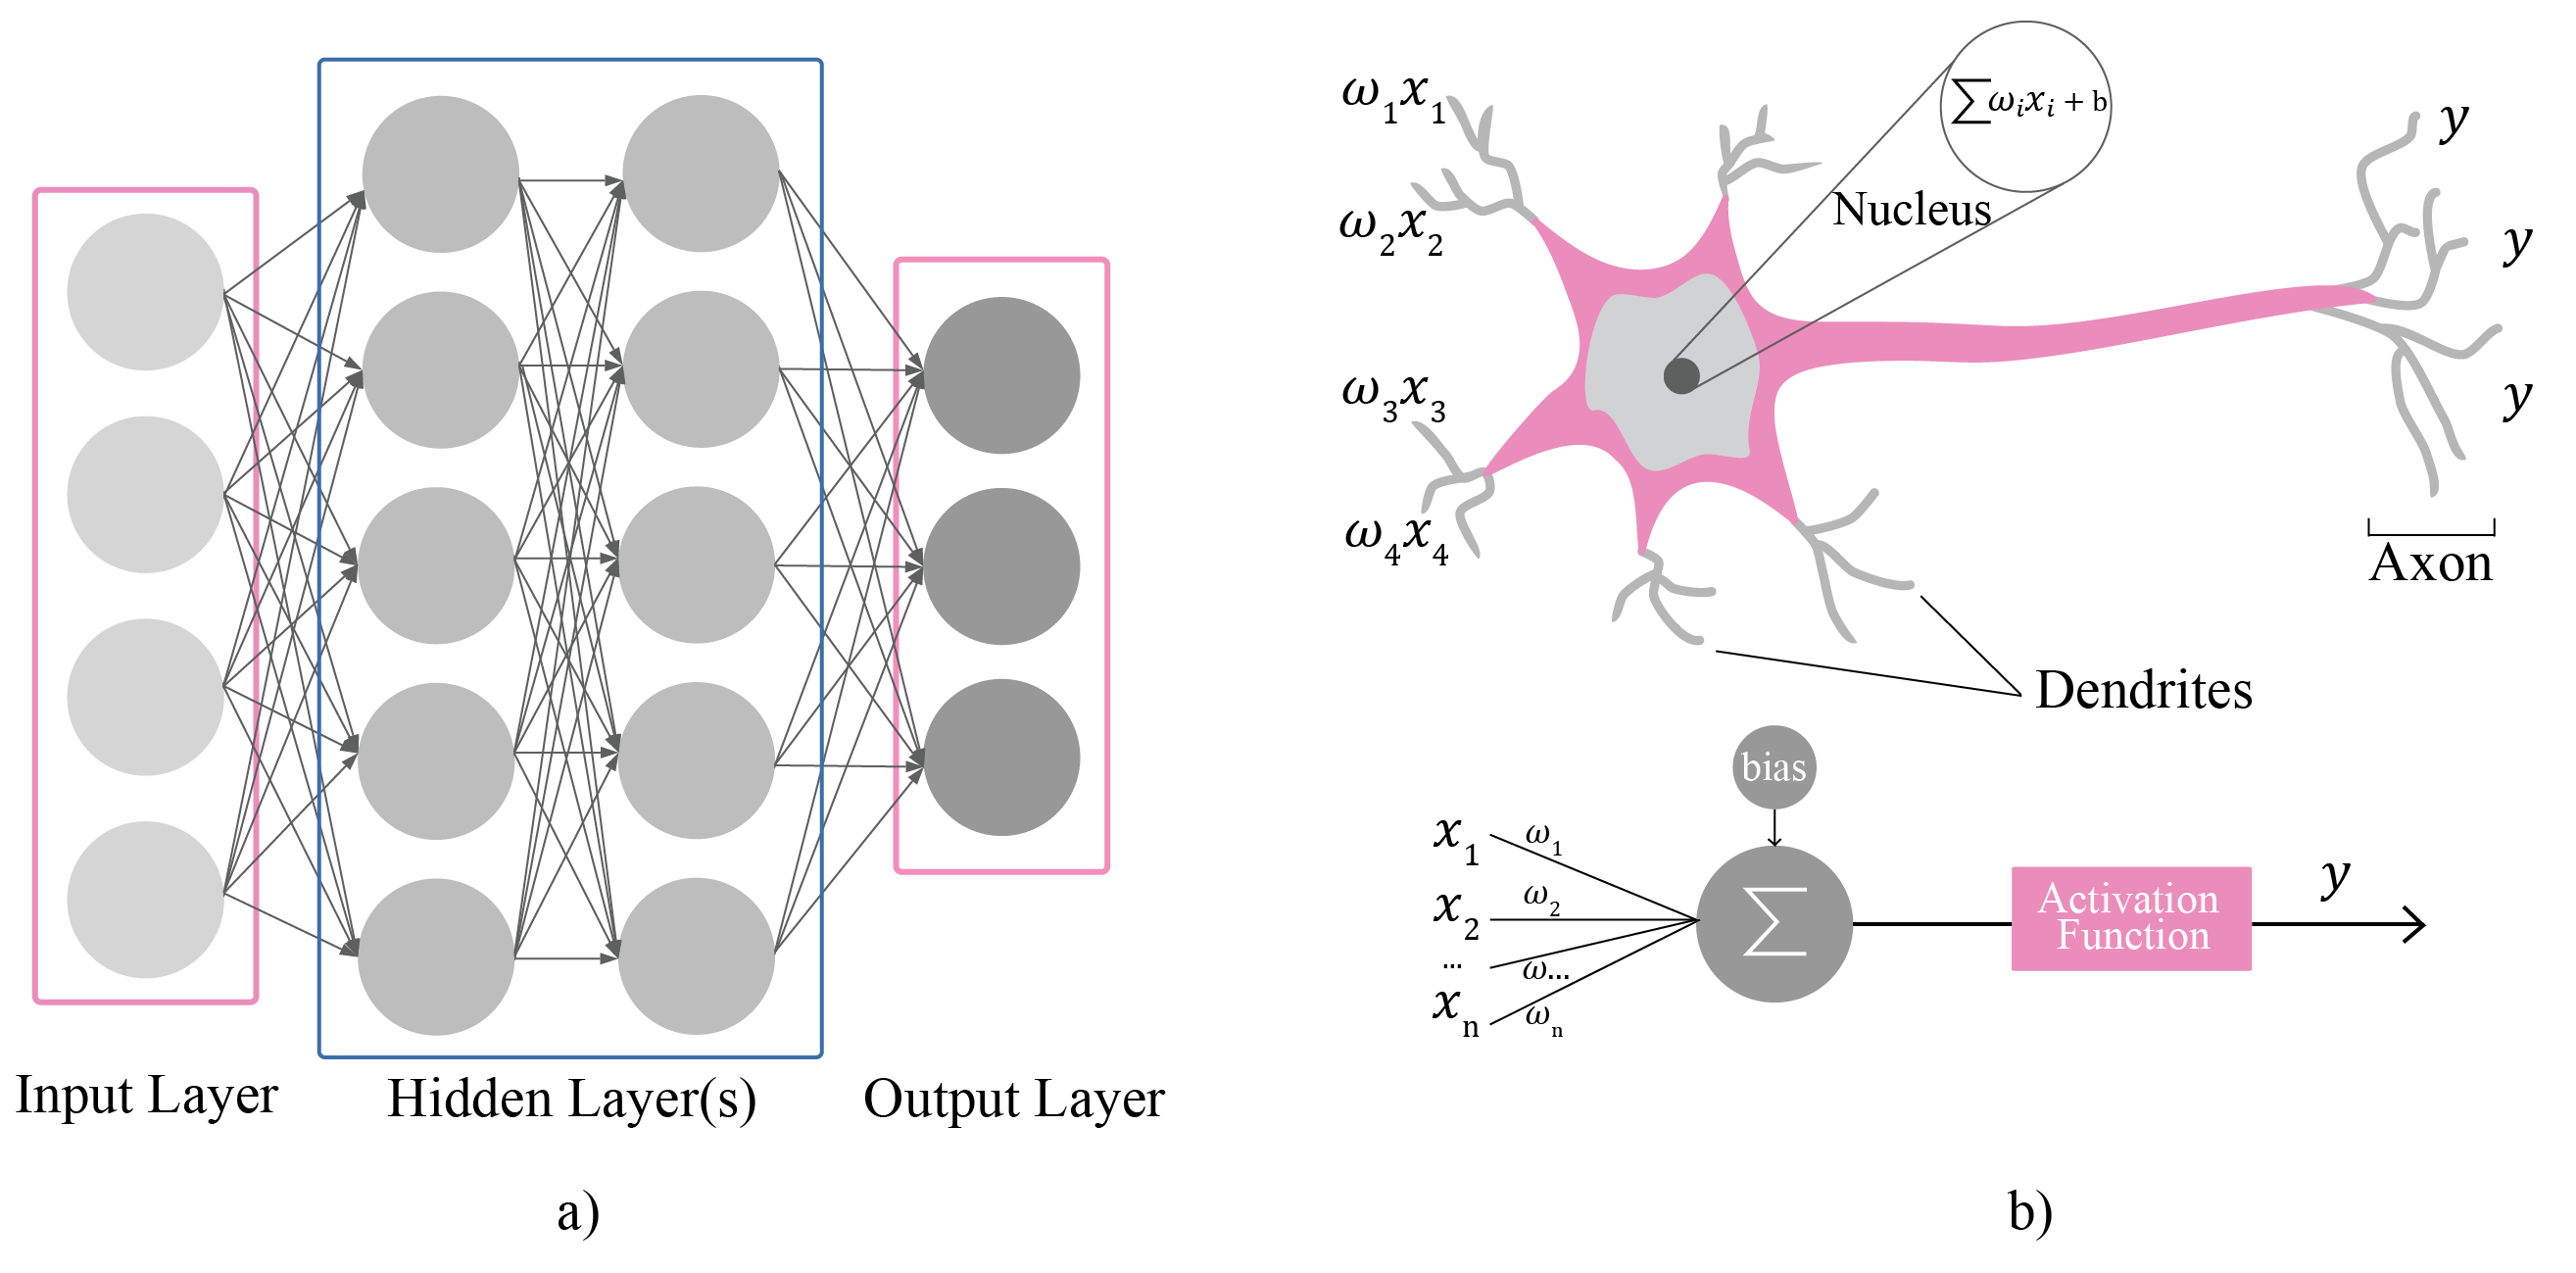
\includegraphics[scale = 0.12]{Chapters/Figures/ANNsfig1.png}}
         \caption{a) Connected Neural Network b) Analogy between biological and artificial neurons.}
         \label{fig:ANNs_fig1}
\end{figure}

As depicted in Figure \ref{fig:ANNs_fig1}, it is possible to understand that similarly to the biological structure, an artificial neuron processes $n$ signals received from $n$ different neurons. The neuron then attributes weight to each of the input signals, representing their importance. The signals are also processed recurring to a bias factor, a scalar that is summed after the weight function. Lastly, the output is formed based on an activation function. A brief description of these functions is presented in the following paragraphs.

\paragraph{2. Activation Funtions}
These functions are responsible for the output $y$ of the neuron. As illustrated in Figure \ref{fig:ANNs_fig1} , their input consists of the weighted sum of the signals and bias factor. As a result, these functions can be generally expressed as 
\begin{equation}
    \label{eq:activation_function_gen}
    y = f (  w x + b ) .
\end{equation}

Activation functions are key in the accuracy of an \gls{ANN} as they directly impact the network's output. Their shape determines the labelling of data points in a dataset, making it crucial to choose the appropriate activation function for a specific dataset, as there is a wide variety available.

As a result, several activation functions have been developed over the years. The simplest one is the linear function in (\ref{eq:activation_function_gen}). However, as mentioned before, sometimes a simple linear function might not be enough to properly distinguish between classes in the dataset. Hence the search for non-linear functions, as the ones presented below. 

\begin{description}

    \item \textbf{Sigmoid:} 
    The sigmoid function is a popular non-linear activation function, defined as 
    \begin{equation}
        \label{sigmoidFuntion}
        \sigma(x) = \frac{1}{(1+ e^{-x})},
    \end{equation}
    that returns values between 0 and 1. Its plot has an S shape as depicted in Figure \ref{fig:sigmoidPlot}.    
    The sigmoid function is not commonly used in deep neural networks due to the vanishing gradient problem \cite{activationFunctions}, which hinders the network's training. This problem can cause gradients to become very small during backpropagation, which makes it difficult for the network to learn by updating its weights, leading to slow convergence or poor performance.  It is caused by the sigmoid function's output being saturating at either 0 or 1, which means that the gradient is close to 0 in those regions. An alternative solution is to use activation functions such as \glspl{ReLU}.
    
     \begin{figure}[ht]
        \centerline{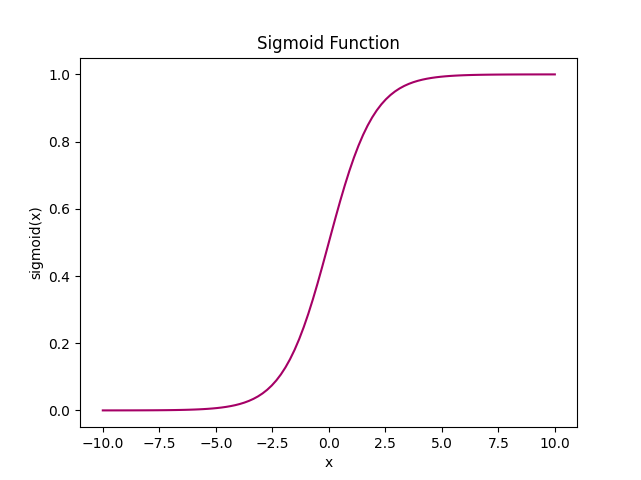
\includegraphics[scale = 0.50]{Chapters/Figures/Sigmoid function.png}}
         \caption{Sigmoid function plot.}
         \label{fig:sigmoidPlot}
    \end{figure}

    \item \textbf{Hyperbolic Tangent:} 
    This function can be described in (\ref{eq:hyperbolicTangent}). However, it's also possible to define it based on the sigmoid function previously introduced, as described in (\ref{eq:hyperbolicTangent2}).
    \begin{equation}
        \label{eq:hyperbolicTangent}
        tanh(x) = \frac{sinh(x)}{cosh(x)},
    \end{equation}
    \begin{equation}
        \label{eq:hyperbolicTangent2}
        tanh(x) = 2sigmoid(2x)-1.
    \end{equation}
    
   \begin{figure}[!h]
        \centerline{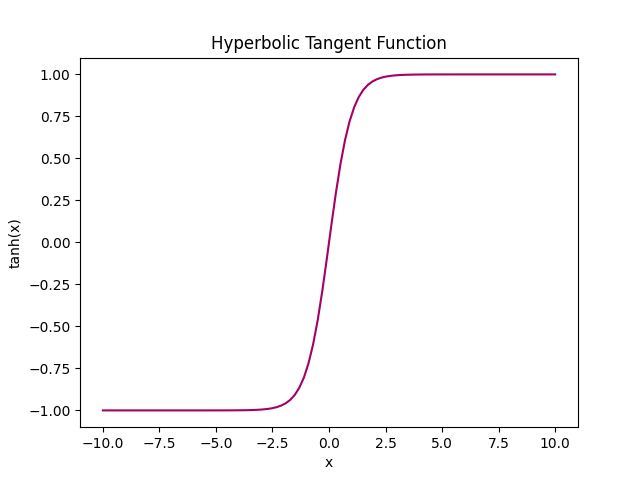
\includegraphics[scale = 0.50]{Chapters/Figures/Tanh function.png}}
         \caption{Hyperbolic Tangent function plot.}
         \label{fig:tanhPlot}
    \end{figure}

    Comparing Figures \ref{fig:sigmoidPlot} and \ref{fig:tanhPlot}, it is possible to see the resemblance between the hyperbolic tangent and the sigmoid functions. Apart from being centered in 0, the similarity makes \textit{tanh} susceptible to the same vanishing gradient problem \cite{activationFunctions}. 
    
          
    \item \textbf{Rectified Linear Unit:}
    \gls{ReLU} is a popular approach for a non-linear activation function. It returns the input if it is positive, and returns 0 if it is negative. The mathematical formula for the \gls{ReLU} function is expressed by
    
    \begin{equation}
        \label{eq:reluFunction}
        y(x) = max(0,x).
    \end{equation}

    As opposed to the previous activation functions, \gls{ReLU} helps alleviate the vanishing gradient problem in deep neural networks. It only has saturation issues in the positive region, making it useful for training the network's weights. The gradient of the ReLU function is always 1 for input values greater than 0. ReLU's plot is depicted in Figure \ref{fig:reluPlot}.    
    
     \begin{figure}[ht]
        \centerline{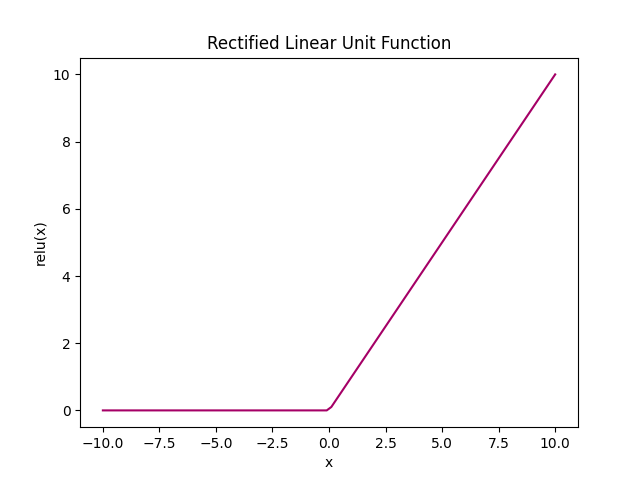
\includegraphics[scale = 0.50]{Chapters/Figures/ReLU function.png}}
         \caption{Rectified Linear Unit function plot.}
         \label{fig:reluPlot}
    \end{figure}
    Furthermore, \gls{ReLU} are considered a breakthrough since they promise cheaper computation than hyperbolic tangent and sigmoid functions and can achieve good performance without relying on unsupervised pre-training \cite{activationFunctions}. However, they are still susceptible to the "dying ReLU" issue, related to the death of some neurons caused by "left-hard-saturation" \cite{activationFunctions}.          

    There have been developed several adaptations of the ReLU such as LReLU, PReLU and RReLU, that can help overcome that issue and enhance the performance of the network. Instead of a null gradient in the negative region, \gls{LReLU} has a small, non-zero value. \gls{PReLU} introduces a learnable parameter that controls the slope of the negative part of the function. \gls{RReLU} also introduces a learnable parameter but it is randomly sampled during training, rather than being learned.

    \item \textbf{Softmax:}
    The softmax function is commonly used in the output layer of neural networks for classification tasks. It is a generalization of the logistic function that allows for more than two classes. Given an input vector of real numbers, the softmax function outputs a vector of $K$ values, where each represents the probability of the input belonging to a particular class. By normalizing the output so that the sum of all the vector's values is 1, it ensures all the values are positive. The function is defined for each neuron $i$ as
    \begin{equation}
        \label{eq:softmaxFunction}
        \sigma (x) = \frac{e^{x_i}}{\sum_k{e^x_k}}.
    \end{equation}    

\end{description}
   
   
\paragraph{3. Training an ANN}
Training an artificial neural network involves adjusting the network's parameters such as the weights and biases of its neurons to minimize the error between the network's predictions and the actual output (or label), for a given set of input data. %This is typically done using an optimization algorithm such as gradient descent. The goal is to find the set of parameters that allow the network to generalize well to unseen data.
It is possible to divide this process into the following stages. First, it is necessary to \textbf{split the dataset} into subsets. 
The use of training, validation, and testing sets aids in evaluating the model's performance, avoiding overfitting, and fine-tuning the model.

Next, the \textbf{output of the network is calculated}. The output represents the prediction of the model for a given input, and by comparing that prediction to the validation subset, it's possible to \textbf{calculate prediction errors}. This can be accomplished with \textit{loss} functions such as Mean Squared Error (MSE), Mean Absolute Error (MAE) and Cross-Entropy.
To minimize the error, \textbf{weights are adjusted} for each neuron in the network through \textit{backpropagation}, which involves propagating the error from the output layer to the input layer.

The output of the network is recalculated, and the described process repeats until either the error is minimized to the smallest value or until an established maximum of iterations is reached.

In summary, training is crucial for improving the accuracy of predictions and building a successful model. This includes avoiding issues such as overfitting and underfitting, which can lead to poor performance. \textit{Overfitting} happens when a model has been optimized for the training data, but has difficulty generalizing to data that is different from the one with which it was trained. \textit{Underfitting} however, reflects a model that is not complex enough to capture patterns in the data, resulting in poor performance on both training and testing data. Proper training can help mitigate these challenges.


\subsubsection{Convolutional Neural Networks}
\label{subsubsec:CNNs}
A \gls{CNN} is a type of deep learning neural network commonly used for image and video recognition tasks since they excel at finding more complex patterns in data. Convolutional, pooling, and fully connected layers constitute a CNN \cite{CNNs_intro}. 

Convolutional layers can extract features from the input image by sliding a filter over it and computing element-wise multiplication between the entries of the filter and the image. These filters are also denoted as kernels and consist of $m$x$n$ matrices. Each convolution results in a new matrix that represents the presence of certain features in the input data, a feature map. The process is repeated for each filter, creating multiple feature maps. 
The convolution operation is defined as:
\begin{equation}
    \label{eq:CNNs}
    S(i,j) = (I*K)(i,j) = \sum_{m} \sum_{n} I (i-m, j-n) K (m,n),
\end{equation}
%
where $I$ represents the input image fed to the \gls{CNN}, K is the kernel and ($i$,$j$) the coordinates of the convoluted image.

The connectivity pattern is different than in standard ANNs: according to \cite{CNNs_intro}, instead of having full connections between layers, kernel functions of reduced dimensions allow neurons in a certain layer to connect only to a specific, limited area of the layer before it.
Because fully connected layers are made up of neurons that connect to every neuron in the layer before them, there are many parameters and a high level of computational complexity. Conversely, \glspl{CNN} are more computationally efficient since neurons only have to learn parameters from a small region of input data. A typical representation of a \gls{CNN} is depicted in Figure \ref{fig:CNN_architecture}.

 \begin{figure}[ht]
        \centerline{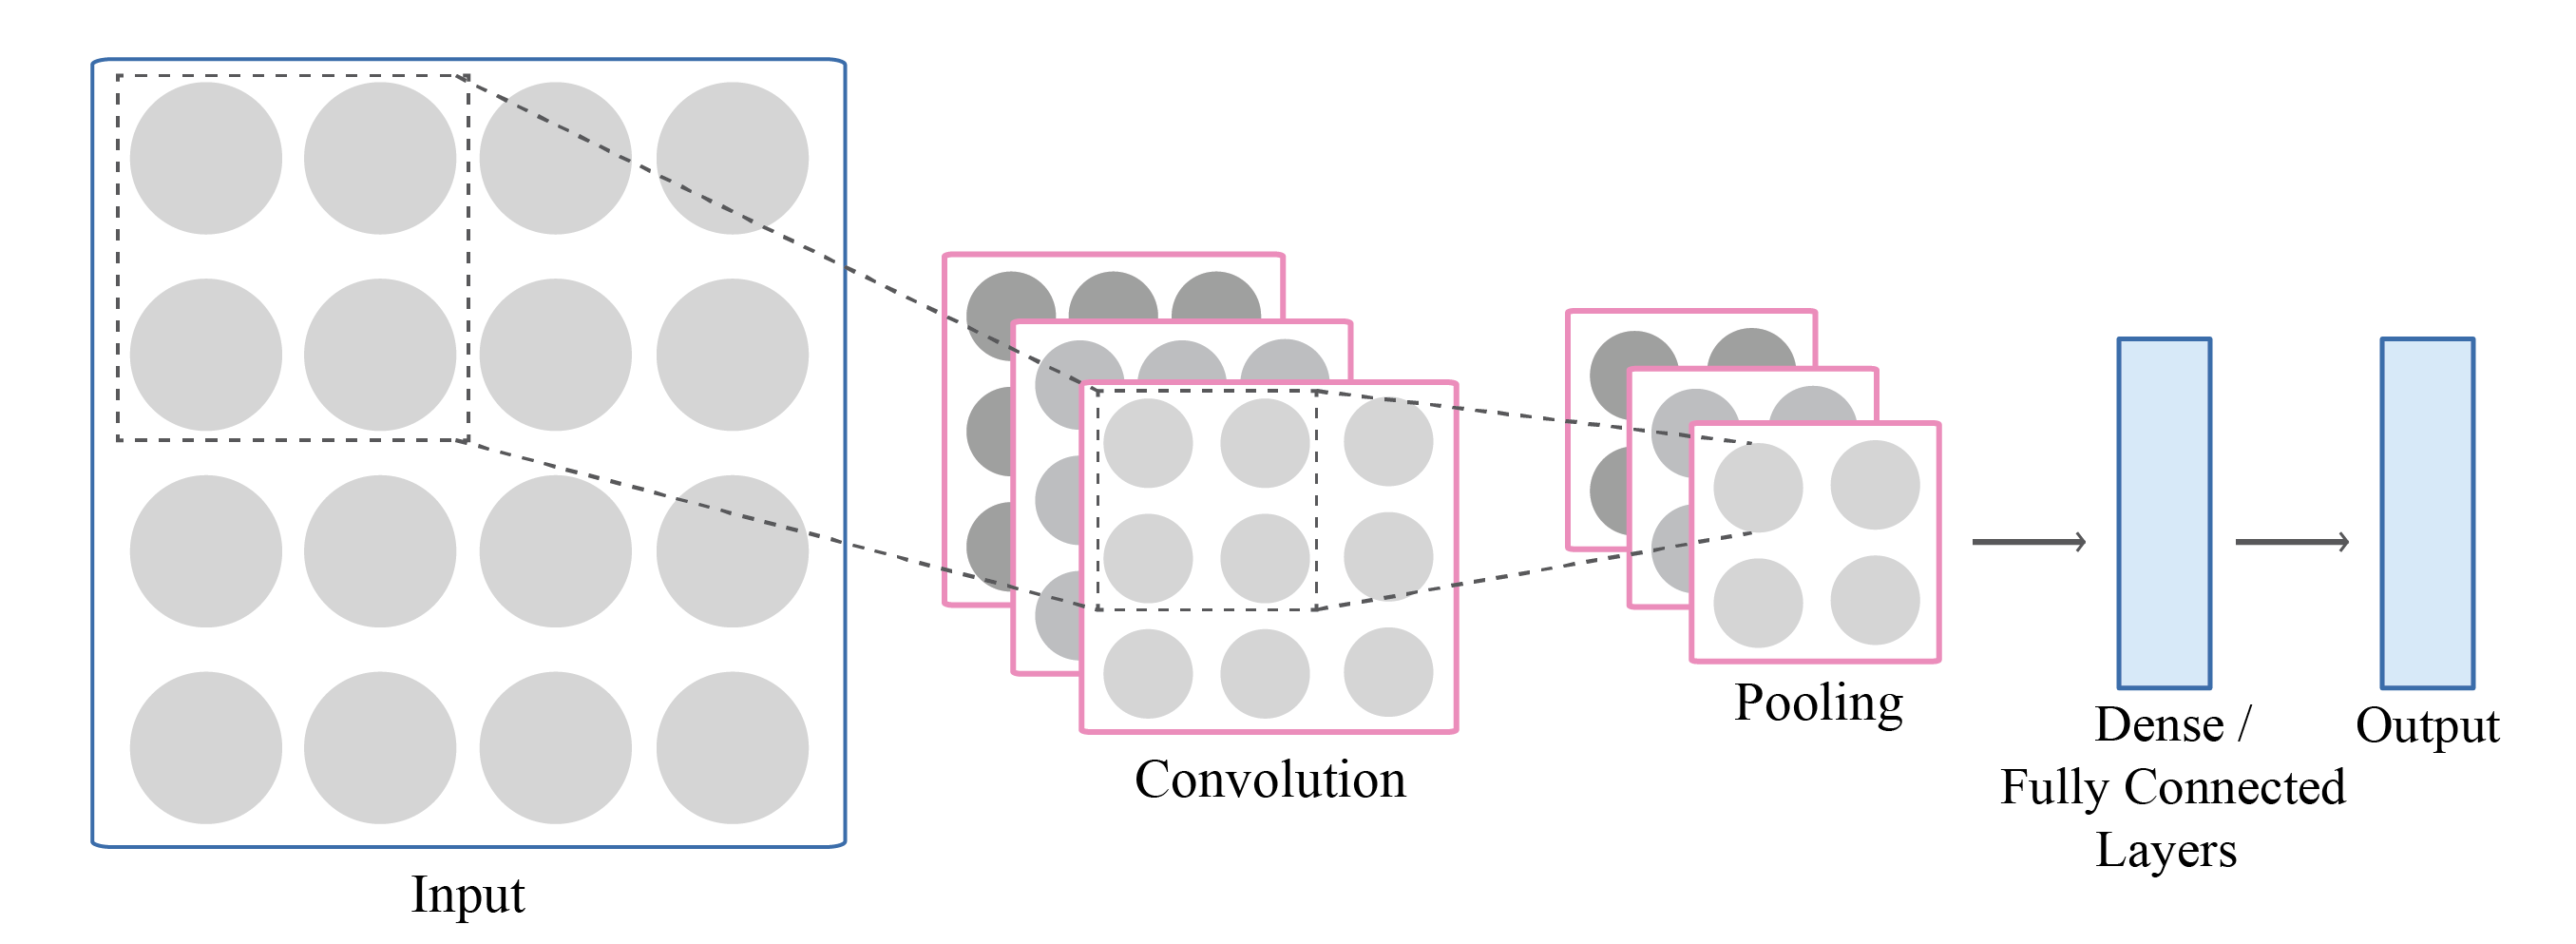
\includegraphics[scale = 0.15]{Chapters/Figures/cnns-02.png}}
         \caption{CNN architecture inspired by \cite{cnnsGraphs}.}
         \label{fig:CNN_architecture}
\end{figure}

Pooling layers are then used to down-sample the feature maps, reducing the dimensionality of the data. They contribute to the model's increased resistance to minor distortions in the input image. This operation can be performed by selecting the maximum value of a region, \textit{max pooling}, or by calculating the average of all values of a region, \textit{average pooling}.

Lastly, fully connected layers or dense layers make predictions based on the processed data, similar to the case of standard ANNs. 


\subsubsection{Recurrent Neural Networks}
\label{subsubsec:RNNs}
\glspl{RNN} are a type of neural network equipped with the capability of processing temporal information by allowing their neurons to exchange information through feedback loops. Thus, neurons can receive feedback from other neurons in the network \cite{RNNs_book}.

RNNs can be unrolled to show a sort of "memory" through time, allowing previous information to persist in the network to help fine-tune further outputs, hence the name "recurrent". This can improve their robustness towards unknown data that differs from training data, reducing the chances of overfitting as well as underfitting.

These networks work especially well with sequential data, such as time series (i.e., a sequence of musical notes in \cite{RNNs}) or natural language, being able to predict the next character in a string \cite{RNNs}, and being useful for tasks such as language translation and speech recognition. Most of these networks can even process sequences with variable lengths.
Figure \ref{fig:RNN_architecture} depicts a typical RNN architecture.

 \begin{figure}[ht]
        \centerline{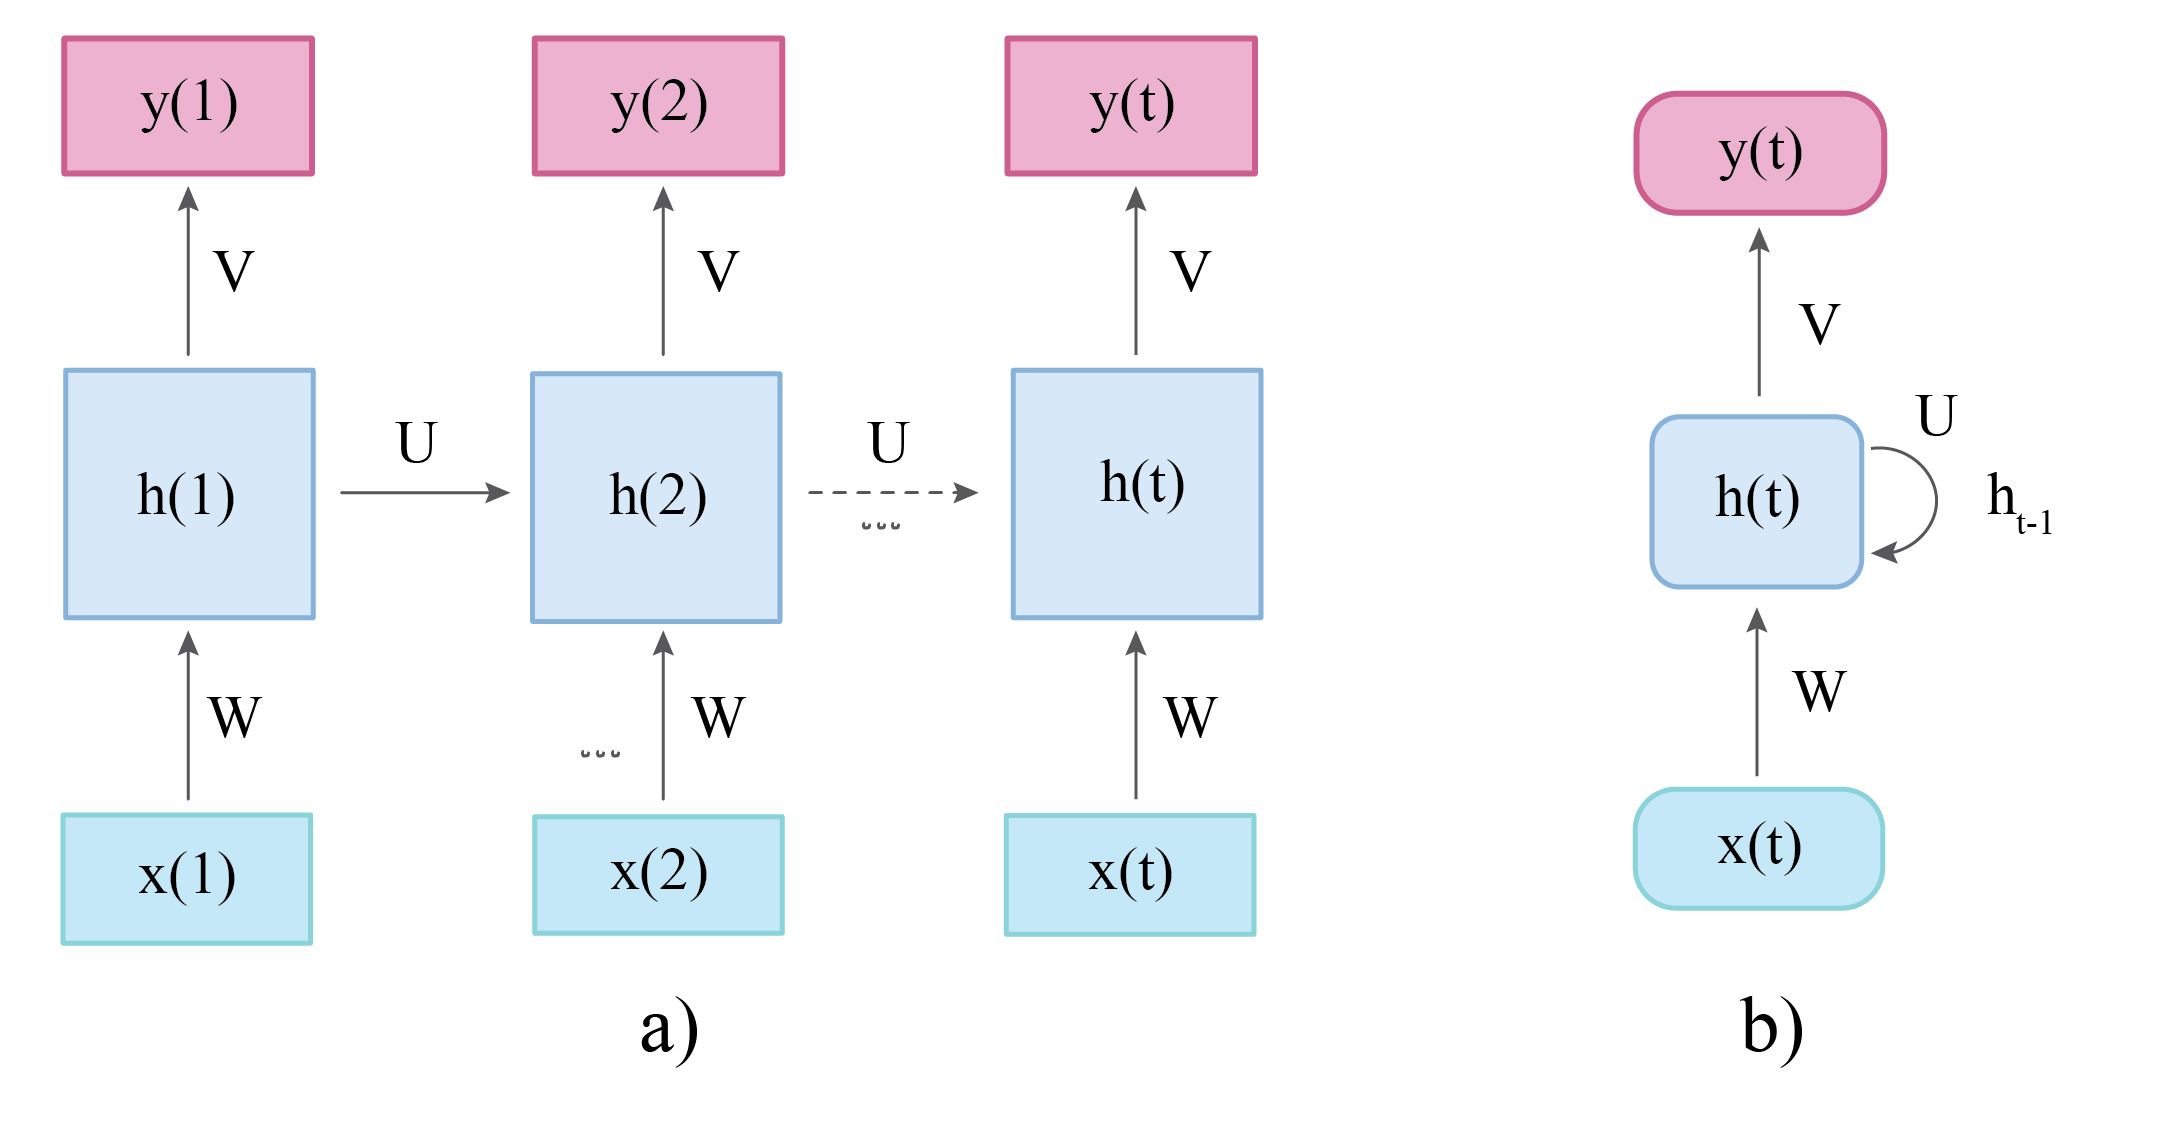
\includegraphics[scale = 0.13]{Chapters/Figures/RNNs_1-02.png}}
         \caption{a) Unfolded RNN architecture b) Folded RNN inspired by \cite{RNNs_tecnico}.}
         \label{fig:RNN_architecture}
\end{figure}

Each RNN cell behaves according to Equations (\ref{eq: RNN1}) - (\ref{eq: RNN3}), where $h(t)$ represents the hidden state, which serves as the network's "memory", and $x(t)$ represents the cell's input at time instant $t$.

\begin{equation}
    \label{eq: RNN1}
    a^{(t)} = b + W h ^{(t-1)} + U x^{t},
\end{equation}
\begin{equation}
    \label{eq: RNN2}
    h^{(t)} = g ( a^{(t)} ),
\end{equation}
\begin{equation}
    \label{eq: RNN3}
    o^{(t)} = c + V h^{(t)} ,
\end{equation}
\begin{equation}
    \label{eq: RNN4}
    y^{(t)} =g ( o^{(t)} ),
\end{equation}

 The Equation (\ref{eq: RNN1}) translates the aggregation of all inputs a cell receives at time step $t$, $a(t)$, which include the new input $x(t)$ and the previous hidden state $h(t-1)$, as well as the bias factor $b$ of the own cell. $W$ and $U$ both represent weight matrices associated with the hidden-to-hidden and input-to-hidden connections. 
 The hyperbolic tangent function is regularly used as an activation function for the output of each cell of the network, thus, in (\ref{eq: RNN2}), the $g$ function can be replaced with $tanh$. Equation (\ref{eq: RNN3}) represents the network's output $o(t)$ at time step $t$, which is dependent on the bias factor $c$ as well as the hidden state $h(t)$ at that moment. Generally, the output of the last layer in the network, the output layer, is submitted to one last activation function $g$, as represented in (\ref{eq: RNN4}). It is common to use the softmax function for this purpose. 
 
The most common type of RNNs are \glspl{LSTM} and \glspl{GRU} since they overcome average RNN problems such as the vanishing gradient and the exploding gradient. The first one has been briefly explained in previous sections. However, exploding gradient refers to the case when the network's weights receive large updates, resulting in an unstable model that cannot learn from data, \cite{RNNproblems1, RNNproblems2}.

\paragraph{Long Short-Term Memory - LSTM}
\gls{LSTM} is a variation of a \gls{RNN} designed to handle long-term dependencies in sequential data. Aiming to overcome the vanishing gradient problem that occurs in traditional RNNs, a special type of memory cell and gates that control the flow of information were created. These allow LSTMs to better maintain information from previous time steps, which makes them ideal for tasks such as language modelling, speech recognition, and time series forecasting. 
Figure \ref{fig:LSTM_architecture} depicts a typical LSTM architecture. 

\begin{figure}[ht]
        \centerline{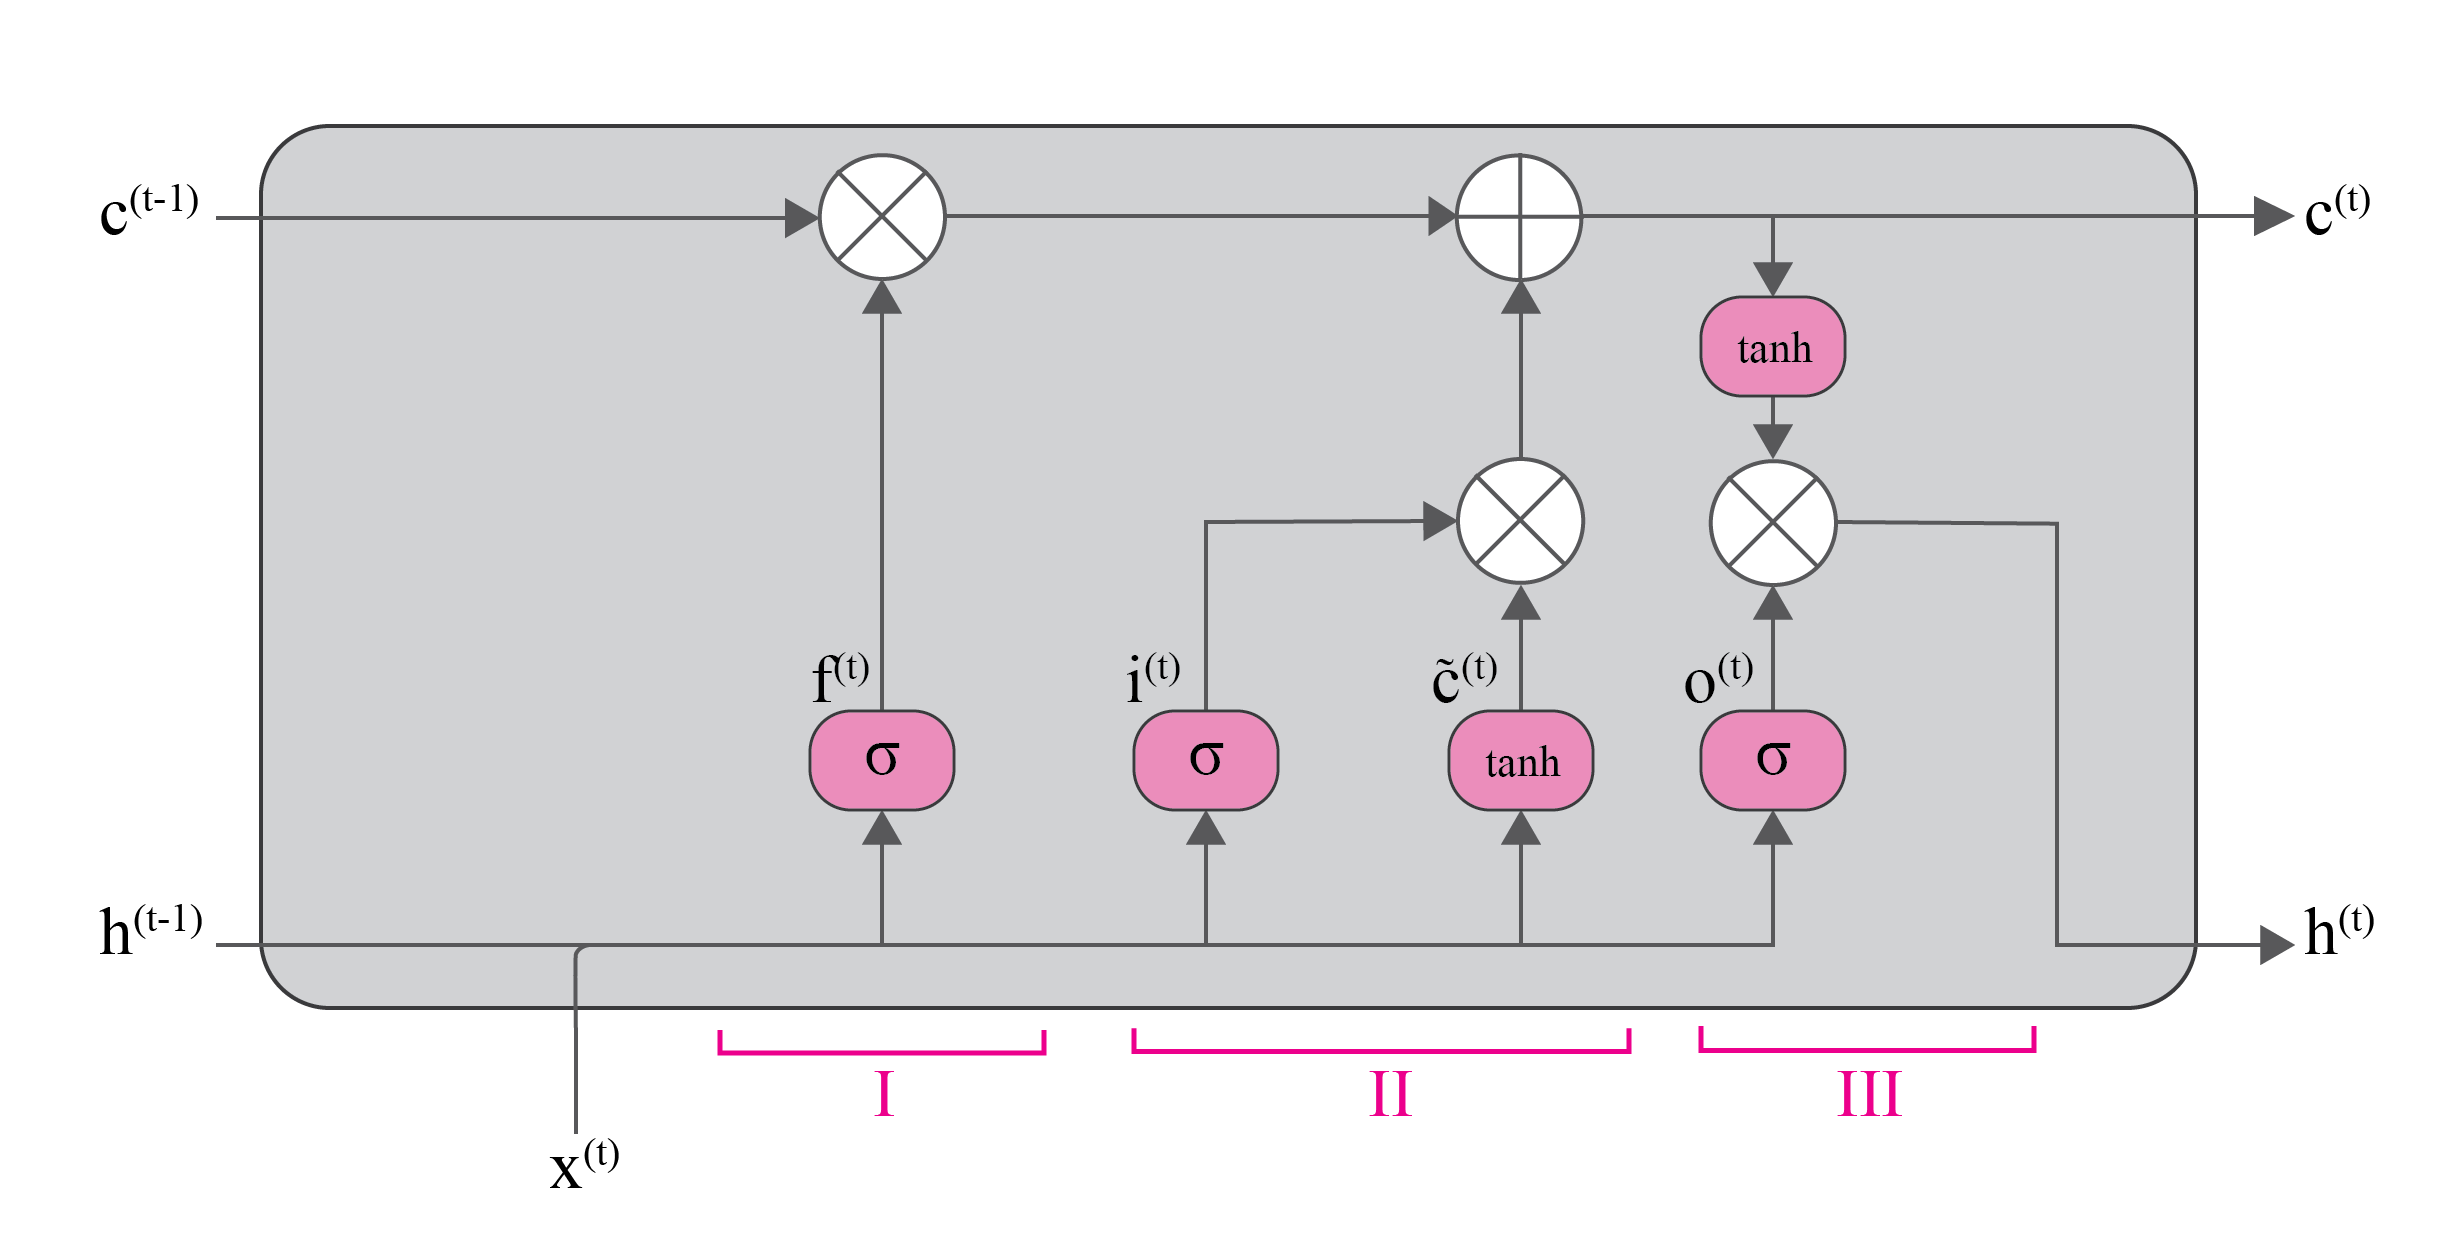
\includegraphics[scale = 0.15]{Chapters/Figures/LSTM-03.png}}
         \caption{LSTM architecture (adapted from \cite{RNNs_tecnico}).}
         \label{fig:LSTM_architecture}
\end{figure}

LSTMs introduce a new concept of cell state, $c(t)$, that is updated at each timestep by a combination of the previous state, the current input, and the output of three different gates (input gate, $i(t)$, forget gate, $f(t)$, and output gate, $o(t)$) in LSTM cell. These gates control the flow of information into and out of the state vector and allow the LSTM to selectively forget or preserve information as it processes the sequence. 
The following paragraphs clarify each of these gates' functions.
\begin{description}

    \item{\textbf{I.}}
    The \textbf{forget gate} constitutes a $sigmoid$ neuron that takes as input the current input $x^{(t)}$ and the previous state $h^{(t-1)}$ and outputs a value between 0 and 1, as described by
        \begin{equation}
            \label{eq:forgetGate}
             f^t =\sigma( W_f \cdot [x^{(t)} , h^{(t-1)}] + b_f ),
        \end{equation}
   where $W_f$ and $b_f$ are weight and biases parameters, respectively. This value is multiplied by the previous state vector, which is scaled by a value between 0 and 1, effectively "forgetting" some of the previous states. This gate plays an important role in allowing the LSTM to focus on the most relevant information and ignore irrelevant or outdated information.

    \item{\textbf{II.}}  
    The \textbf{input gate} is responsible for controlling the flow of information into the cell's state vector. It is a $sigmoid$ neuron that also receives the current input and the previous state, and outputs a value between 0 and 1. Its operation is described by
    \begin{equation}
        \label{eq:inputGate}
        i^t=\sigma( W_i \cdot [x^{(t)} , h^{(t-1)}] + b_i ),
    \end{equation}
    where $W_i$ and $b_i$ are weight and biases parameters, respectively. 
    This output will be multiplied by possible candidate values, $c(t)$, which result from the following expression
    \begin{equation}
        \label{eq:cellState candidate}
         \tilde c^t=\tanh( W_c \cdot [x^{(t)} , h^{(t-1)}] + b_c),
    \end{equation} 
    where $W_c$ and $b_c$ are weight and biases parameters. 
    Lastly, the result of this operation is summed with the result of the forget gate, resulting in the \textbf{cell state} for the current time step. It can be characterized by the following expression
    \begin{equation}
        \label{eq:cellState}
         c^t= f^{(t)} * c^{(t-1)} + i^{(t)} *  \tilde c^t,
    \end{equation} 
    where $*$ denotes the Hadamard product.
    
    \item{\textbf{III.}} 
    The \textbf{output gate} influences what information is shared from the cell state to the hidden state, and consists of a $sigmoid$ neuron which also takes the current input and the previous state as input and outputs a value between -1 and 1, as described by the following expression
        \begin{equation}
            \label{eq:outputGate}
            o^{(t)} =\sigma( W_o \cdot [x^{(t)} , h^{(t-1)}] + b_o ),
        \end{equation}
    where $W_o$ and $b_o$ are the weight and biases parameters, respectively.
    
    The result of this operation it then multiplied with the output oh the hyperbolic tangent applied to the current cell state, $c(t)$, resulting in the   \textbf{hidden state} as described by the following equation:
          \begin{equation}
            \label{eq:hiddenState}
            h^{(t)} =o^{(t)} * \tanh( c^{(t)}).
        \end{equation}  
\end{description}

\paragraph{Gated Recurrent Unit - GRU}
\glspl{GRU} were first introduced in \cite{GRUs_Cho2014}, were the first to describe , with the goal of eliminating the vanishing gradient problem. \glspl{GRU} are one of many variations on traditional LSTMs that differ from the original by combining the cell state and hidden state, as well as the forget and input gates into a single update gate. GRU's architecture is depicted in Figure \ref{fig:GRU_architecture}, where the only gates are the reset and update gates.
\begin{figure}[ht]
        \centerline{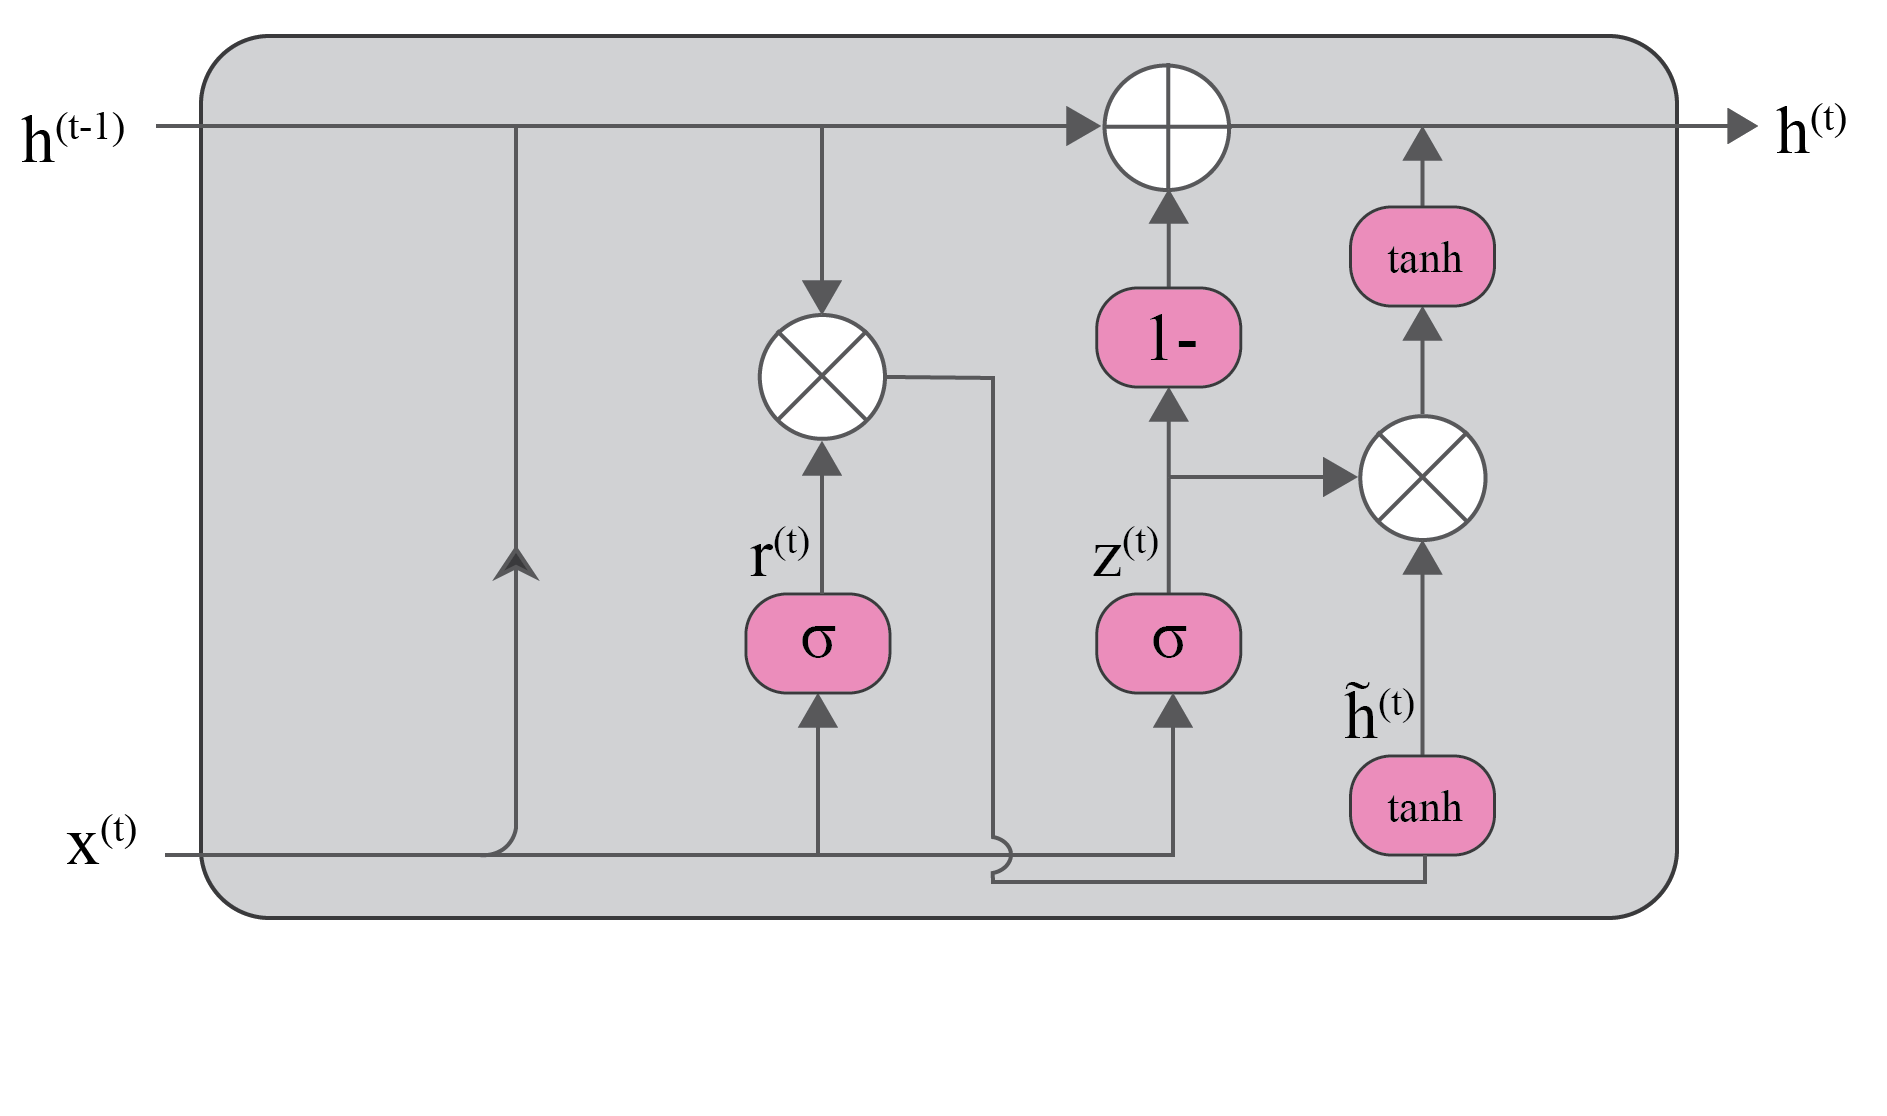
\includegraphics[scale = 0.15]{Chapters/Figures/GRU-04.png}}
         \caption{GRU architecture (adapted from \cite{RNNs_tecnico}).}
         \label{fig:GRU_architecture}
\end{figure}
The \textbf{reset gate} can select what information to discard from the previous hidden state, as described by
      \begin{equation}
        \label{eq:resetGate}
        r^{(t)} =\sigma ( W_r \cdot [h^{(t-1)}, x^{(t)}] + b_r),
    \end{equation}  
where $W_r$ and $b_r$ are weight and biases parameters, $h^{(t-1)}$ is the hidden state of the previous time step and $x^{(t)}$ is the current input vector.
The other gate, \textbf{update gate} $z^{(t)}$, has the contrary function: it selects which information gets to flow into the hidden state vector. Its operation is described as
      \begin{equation}
        \label{eq:updateGate}
        z^{(t)} =\sigma ( W_z \cdot [h^{(t-1)}, x^{(t)}] + b_z),
    \end{equation} 
where $W_z$ and $b_z$ are weight and biases parameters. 
A vector containing a list of possible candidates to add to the hidden state is given by
      \begin{equation}
        \label{eq:hiddenStateCandidates}
        \tilde h ^{(t)} =\tanh ( W_h \cdot [h^{(t-1)}, x^{(t)}] + b_h),
    \end{equation} 
where $W_h$ and $b_h$ are the learnt weights and biases. 
Finally, the current hidden state can be calculated based on the following expression
      \begin{equation}
        \label{eq:hiddenStateGRU}
         h ^{(t)} = (1- z^{(t)}) * h^{(t-1)} + z^{(t)}* \tilde h ^{(t)},
    \end{equation} 
where $*$ denotes the Hadamard product.

In conclusion, while the architecture of GRUs is significantly simpler than that of LSTMs, their performance can be quite similar \cite{GRUs_Cho2014}. GRUs may be preferred due to their faster computation time, whereas the latter may be preferred due to slightly higher accuracy.


\subsubsection{Generative Adversarial Networks}
\label{subsubsec:GANs}
A \gls{GAN} is a neural network architecture composed of two components: a generator network and a discriminator network. The generator creates new data samples synthesized from the learned distribution of training data, hence the name "\textit{generative}", whereas the discriminator network attempts to tell generated and real samples apart. The two networks are trained in an adversarial process in which the generator attempts to build samples that will deceive the discriminator, which attempts to correctly identify the generated samples. A simple analogy is illustrated in \cite{GANS_ieee}, where these two entities are compared to an "\textit{art forger} and an \textit{art expert}". A typical GAN architecture is depicted in Figure \ref{fig:GANsArchitecture}.
\begin{figure}[ht]
        \centerline{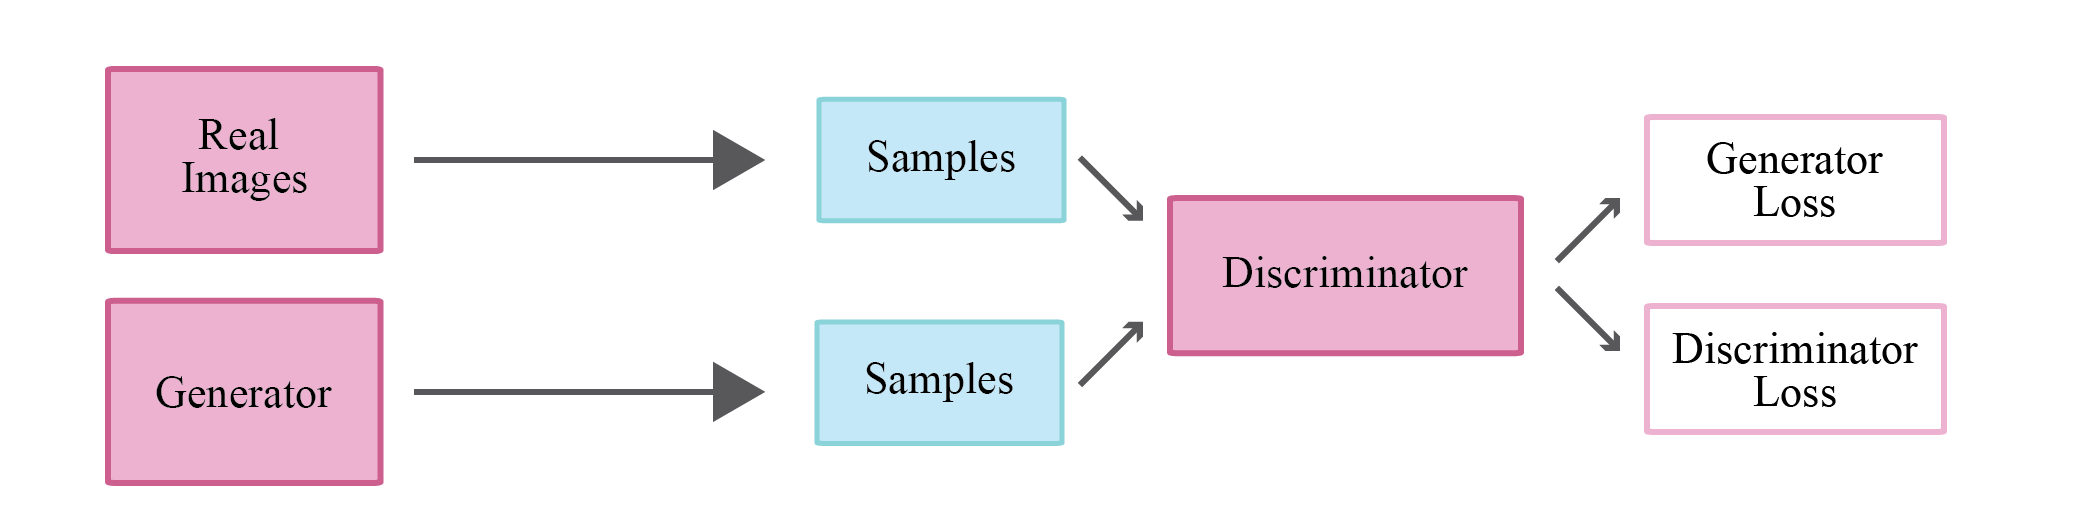
\includegraphics[scale = 0.15]{Chapters/Figures/GANS-05.png}}
         \caption{GAN architecture (adapted from inspired by \cite{GANSgoogle}).}
         \label{fig:GANsArchitecture}
\end{figure}

Training a GAN entails two distinct training processes. Training the discriminator is similar to training a simple classifier, which uses discriminator loss to penalize the discriminator each time it classifies a sample incorrectly. Both network's weights are updated using backpropagation based on the discriminator loss and generator loss. To train the generator, random noise is fed into it and transformed into a data instance. The discriminator then tries to sort the data, deciding if it is true or false, and the generator's loss is calculated using the discriminator's output. It is worthy to note that these two processes are alternatively repeated.

GANs are used for a wide range of tasks, including image synthesis, image-to-image translation and image superresolution \cite{GANS_ieee}. However, they still suffer from a common problem across deep learning models,  the vanishing gradient problem: if the discriminator executes its job perfectly, the generator's training may fail. The mode collapse issue can also occur when a generator produces a limited set of outputs that are always accepted by the discriminator, causing both the generator and discriminator to get stuck in a local minimum, leading to reduced diversity in generated outputs. Failure to converge can also happen in GANs if the generator excels at creating perfect samples, leading the discriminator to fail at distinguishing between real or fake samples. There are ways to remedy those issues, as discussed in \cite{GANSgoogle}.

\subsubsection{Auto Encoders}
\label{subsubsec:autoEncoders}
An autoencoder is a neural network in the field of unsupervised learning that is composed of an encoder and a decoder. The first learns to map input data into an internal and compact representation, and then the latter decodes it as accurately as possible, forming an output similar to the original data. The encoder and decoder are trained so that the discrepancy between the original input and the reconstructed output is reduced.
With autoencoders it is possible to have outputs of the same dimension as inputs, their architecture is depicted in Figure \ref{fig:AutoencoderArchit}.
\begin{figure}[ht]
        \centerline{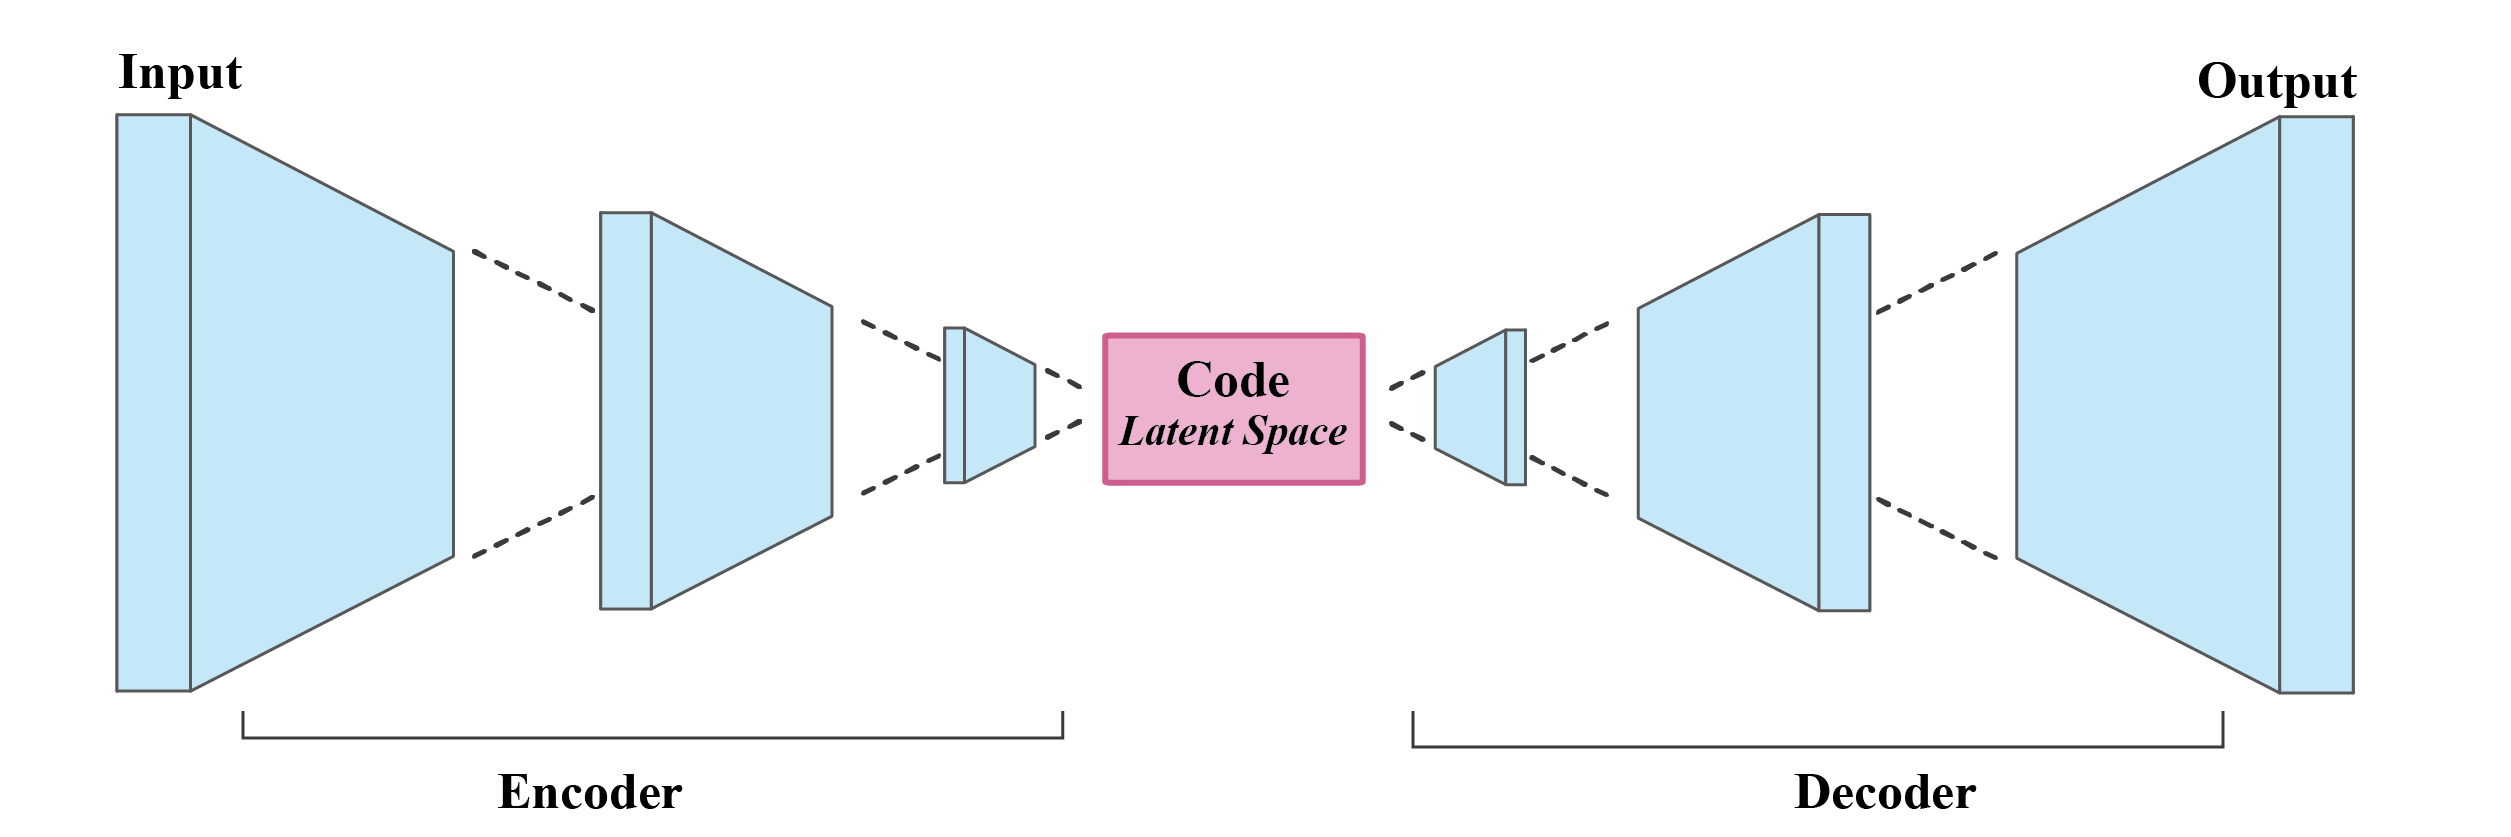
\includegraphics[scale = 0.15]{Chapters/Figures/Autoencoder-06.png}}
         \caption{Autoencoder architecture.}
         \label{fig:AutoencoderArchit}
\end{figure}

The encoder generates code that gathers important features from input data, hence AEs can be compared to a generalization of the PCA algorithm, \cite{autoencoders}, also being useful for feature extraction approaches. 
Some AEs can be used as generative models, while others can be used to improve classification by performing feature extraction. AEs can also be used for anomaly detection and dimensionality reduction, \cite{autoencoders}.



\section{State of the Art / Related Works}
\label{sec:related_works}

Some work has already been done in the area of \gls{RF} sensing, namely for the purpose of human motion detection. A brief summary of some of this work will be presented in the next paragraphs, for a better understanding of the developments made so far, as well as to identify open challenges in RF sensing. The study of several works available in the literature also proved to be important to recognize the performance of some technologies mentioned throughout the sections of this chapter when applied to the human motion detection context.

 In \cite{SOA_FMCWtempofeature}, S. J. Ryu et al. introduce feature-based gesture recognition in a \gls{FMCW} radar system. A \gls{RDM} is obtained from raw signals of FMCW radar and a variety of features are generated from it. The \gls{QEA}, a wrapper-based algorithm, was employed for feature selection, along with an \textit{Information Factor} based on the \gls{mRMR}. This combination, \gls{QEA-IF}, proved to be helpful in recognizing feature subsets related to gesture recognition, which were more useful and generally improve the accuracy of the predictions up to 85.29\%. It is worth noting that the authors identified that the shape of the \gls{RDM} map had little to no effect on gesture recognition and that intensity information was more useful for their implementation than range and velocity information. Therefore, the intensity of the most reflective point of the signal, $\rho^*$, and the total energy of received signals, $E_{inst}$, were identified as relevant features. Furthermore, a comparison between the performance of \gls{QEA-IF} and other classifiers such as \textit{KNN} and \textit{Random Forest} also concluded that QEA-IF achieves better accuracy and faster recognition rate.

 A research study on gesture recognition using a 77 GHz FMCW radar system was conducted by Y. Sun et al, \cite{SOA_microDoppler_fmcw}, where the system utilizes micro-Doppler ($\mu$D) signatures to recognize driver's gestures for an in-vehicle driver monitoring application. Because these signatures were frequently distorted by the presence of multiple moving targets, and the goal was to recognize only the driver's hand gestures, range information was included to filter out the influence of irrelevant moving targets. 
The authors proposed a method using five handcrafted features and a \gls{KNN} classifier, achieving an average prediction accuracy of 83.52\%. However, for three of the gestures, the accuracy was 90\%, while for the remaining two, which required more axial movement, the accuracy was only 63\%. This is likely due to the radar's sensitivity to radial movements and lack of information on axial movements. The authors also discussed potential future research to address issues with wideband background noise and to implement feature selection methods such as PCA to improve training efficiency.

In \cite{SOA_Magnitude_Phase_Features}, P. Goswami et al. describe a low-complexity multi-gesture classification solution for consumer and automotive electronics that employs a 77 GHz mm-wave low-power CMOS radar, as well as an innovative algorithm and software pipeline. It enables real-time gesture detection and uses an \gls{ANN} for classification, using magnitude and phase-based features, as well as statistical features.  Overall, 96\% accuracy for 6 gestures was achieved across 8 users, which is an interesting result for a single-chip radar solution with limited memory, computation power, and angle resolution constraints. 

In \cite{SOA_DRDTmap_features}, C. Ding et al. proposed a method for recognizing continuous human motion using radar technology, specifically a \gls{FMCW} radar system. The method, called \gls{DRDT}, extracts relevant information from range-Doppler frames obtained from the radar's signals. Then, using a peak search method, each human motion is located and separated, and multidomain features are extracted. These time, range, Doppler and RCS (radar cross section) features are fed to a \gls{KNN} classifier, resulting in robust recognition accuracy of around 95\% for single motions and 91.9\% for continuous motions. Although the model performed well across various angles, individuals, and different distances and directions, allowing real-time recognition of human motion in real-living environments, the authors observed a slight deterioration in performance beyond a 30° view angle.

The work in \cite{SOA_datasetPortability} presents results for a FMCW radar that uses micro-Doppler signatures for fall detection. The researchers extract micro-Doppler signatures from radar signals and use transfer learning (\textit{AlexNet}), \gls{SVM},\gls{KNN}, and deep learning (\textit{GoogleNet}) algorithms to automatically extract features and perform classification, respectively. The experiment involves several people performing six different activities in four different locations. The central idea is to create a generalized fall detection system that works regardless of location or subjects involved, which entails investigating the portability and applicability of radar datasets for \gls{HAR}. All three classifiers produced significant results, with an average test percentage accuracy of 78.25\% for SVM, 77.15\% for KNN, and 74.7\% for GoogleNet. Researchers stated that further developments could be pursued by taking more measurements in different locations and involving elderly people, with the aim of improving the test accuracy.

The use of RADAR sensors in short-range human monitoring applications, such as activity classification in smart homes and gesture recognition for human-computer interaction is discussed in \cite{SOA_FMCW_biLSTM}. Similar to other works, micro-Doppler signatures and range-time information are extracted from radar signals. For classification, a \gls{Bi-LSTM} network is used, and unlike most related works that use \glspl{CNN}, it interprets radar data as a temporal series rather than images. The ability to analyze these sequences, according to the authors, is one of their main contributions, allowing for more realistic data acquisition. Furthermore, they proposed a stacked \gls{Bi-LSTM} system that is better suited to the temporal sequence nature of the data and achieves over 90\% accuracy for 45 different activity sequences tested.

J. Bhatia et al., \cite{SOA_1DFFT_freqFeatures}, adopted an FMCW radar to build a detection system that can distinguish between drones, humans, and cars. A range FFT plot is created based on the radar signals, and the authors claim that this is the first project relying on range FFT features to perform target classification.  Two lightweight classification models, such as Logistic Regression and Naive Bayes, are explored to assess the performance. The selected features fed to the ML algorithms were based on the peaks detected in those plots, some of which included width, area, and standard deviation of peak values. Overall, Logistic Regression and Naive Bayes algorithms reached 86.9\% and 73.9\% accuracy, respectively, and the researchers note that some future work could be done to improve target size and shape detection and that range-Doppler plots could be introduced for more reliable classification. It should be noted that this paper contributes to advancements in efficient and dependable management of ground station traffic at a cost-effective price point as well as computer vision and object recognition.

In \cite{SOA_phaseExtraction}, K. Han et al. propose a phase-extraction technique for a \gls{FMCW} radar that allows the detection of target motions. The technique involves decomposing an FMCW chirp signal into multiple-frequency signals, 250 to be exact, to extract modulated phases due to target motions. This novel method can extract the phase without performing a \gls{FFT}, which can overcome the range migration problem that causes errors in phase extraction using a conventional FFT-based method. It reduces noise and can improve detection accuracy for both human vital signals, which consist of small vibrations, and several body motions. Thus, the detection of phase can be precise regardless of the type of moving targets.

R. Cruz et al. \cite{Cruz2022} studied the importance of various features in classifying human mobility scenarios using an \gls{RF} sensing system in the 76-81 GHz band. The authors compared the performance of different features computed from the RF time of flight and use four different methodologies to evaluate their importance: \gls{MI}, \gls{ANOVA}, the feature weighting algorithm \textit{RelieF}, and \gls{RFE}. Overall, 126 raw features were submitted to each feature selection method and gls{KNN} was used as a classifier. Despite all methodologies being capable of identifying features of lower importance, it was concluded that RFE leads to better accuracy in classification when its 18 selected features are used for classification. ANOVA demonstrated the lowest accuracy rate, and even PCA could not surpass RFE when  the number of selected features was higher than 12.


